% Dokumentation DIFA
% Kompilieren: pdflatex Dokumentation.tex (zweimal ausführen fuer Verzeichnisse)
% Struktur: siehe Dokumentation_Aenderungen.md
% Stellen mit \todo{...} sind noch auszufuellen.

\documentclass[11pt,a4paper]{article}

\usepackage[utf8]{inputenc}
\usepackage[T1]{fontenc}
\usepackage[ngerman]{babel}
\usepackage{lmodern}
\renewcommand{\familydefault}{\sfdefault}
\usepackage[a4paper,margin=2.5cm]{geometry}
\usepackage{graphicx}
\usepackage{booktabs}
\usepackage{tabularx}
\usepackage{longtable}
\usepackage{xcolor}
\usepackage{listings}
\usepackage{enumitem}
\usepackage{setspace}
\usepackage{fancyhdr}
\usepackage{caption}
\usepackage{tikz}
\usetikzlibrary{arrows.meta,positioning}
\usepackage[hidelinks]{hyperref}

\onehalfspacing
\emergencystretch=3em
\setlength{\parindent}{0pt}
\setlength{\parskip}{0.6em}

% Kopf- und Fusszeile
\pagestyle{fancy}
\fancyhf{}
\fancyhead[L]{Dokumentation DIFA}
\fancyfoot[C]{Seite \thepage}
\renewcommand{\headrulewidth}{0.4pt}

% Platzhalter-Markierung
\newcommand{\todo}[1]{\textcolor{red}{[TODO: #1]}}

% Code-Darstellung (Prompts, Befehle)
\lstset{
  basicstyle=\ttfamily\small,
  breaklines=true,
  frame=single,
  backgroundcolor=\color{black!4},
  columns=fullflexible,
  keepspaces=true,
  literate=%
    {ä}{{\"a}}1 {ö}{{\"o}}1 {ü}{{\"u}}1
    {Ä}{{\"A}}1 {Ö}{{\"O}}1 {Ü}{{\"U}}1
    {ß}{{\ss}}1 {–}{{-{}-}}1
}

\begin{document}

% ------------------------------------------------------------
% Titelblatt
% ------------------------------------------------------------
\begin{titlepage}
  \centering
  \vspace*{2cm}
  {\large Berner Fachhochschule\par}
  \vspace{0.3cm}
  {\large Wirtschaft\par}
  \vspace{3cm}
  {\Huge\bfseries Dokumentation DIFA\par}
  \vspace{0.8cm}
  {\Large Aktualisierung, mehrsprachige Suche und Themenbereich Regulatory Compliance\par}
  \vspace{3cm}
  {\large Studiengang: Wirtschaftsinformatik\par}
  \vspace{1cm}
  {\large Yannic Reust\par}
  \vspace{0.5cm}
  {\large Experte/Expertin: Gimeno Raúl Diego\par}
  \vspace{0.5cm}
  {\large Datum des Einreichens: 15.11.2026\par}
\end{titlepage}

% ------------------------------------------------------------
% Abstract
% ------------------------------------------------------------
\pagenumbering{roman}
\section*{Abstract}
Die Webplattform „CS-UBS-Fusion“ dokumentiert die Übernahme der Credit Suisse durch die UBS und besteht aus Fallstudien, Blogbeiträgen und einem Organigramm. Im Modul DIFA wurde sie in drei Aufgaben weiterentwickelt. Erstens wurde die App von Next.js 15.5.9 auf 16.3.2 und Prisma von 6.17.1 auf 6.19 aktualisiert, weil Prisma 7 MongoDB nicht unterstützt. Die Aktualisierung wurde mit einem Vergleich von selbst geschriebenen und KI-optimierten Prompts dokumentiert. Zweitens wurde das bisher funktionslose Suchfeld im Header zu einer mehrsprachigen Suche über Fälle, Blogs und Organigramm ausgebaut, mit Vorschlägen während der Eingabe, Hervorhebung, Tippfehlertoleranz und Tastaturbedienung. Drittens entstand der Themenbereich „Regulatory Compliance“ mit eigener Navigation, Übersichtsseite, vier Platzhalterseiten und einer Kapitel-7-Seite mit Diagrammen und Tabellen zu den Kapitalquoten der Credit Suisse.

Die Arbeit entstand mit KI-Unterstützung: Claude Code diente der Planung und Codierung, die Modelle Qwen3.5 und Mistral der Überprüfung des Codes. Die Aufgaben wurden in eigenen Git-Branches bearbeitet, bei Aufgabe 3 teilweise parallel mit mehreren Agents. Die Resultate wurden mit Build, manuellen Tests im Browser und, bei der Suche, mit 23 automatisierten API-Tests geprüft. Alle drei Aufgaben sind umgesetzt. Als wichtigste Erkenntnis zeigte sich, dass ein vollständiger Prompt mit Ist-Zustand, Ziel und Rahmenbedingungen sowie ein Plan vor der Umsetzung die Qualität der KI-Ergebnisse stark verbessern.

\clearpage
\tableofcontents
\clearpage
\pagenumbering{arabic}

% ------------------------------------------------------------
% 1 Einleitung
% ------------------------------------------------------------
\section{Einleitung}

\subsection{Projektkontext}
Die vorliegende Arbeit entstand im Modul DIFA (Digital Finance – Anwendung und Technologien, HS26) an der Berner Fachhochschule, im dritten Semester des Studiengangs Wirtschaftsinformatik. Ausgangslage ist die bestehende Webplattform „CS-UBS-Fusion“, die die Übernahme der Credit Suisse durch die UBS redaktionell dokumentiert und begleitet. Sie besteht aus den drei Inhaltsbereichen Fallstudien, Blogbeiträge und Organigramm und ist mehrsprachig (Deutsch, Englisch, Französisch, Spanisch, Italienisch). Die Arbeit wurde vom Experten Raúl Diego Gimeno in drei aufeinanderfolgenden Aufgaben gestellt und begleitet. Die Aufträge wurden schrittweise vergeben; der Originaltext steht im Anhang~\ref{app:auftrag}.

\subsection{Zielsetzung und Überblick über die drei Aufgaben}
\begin{itemize}
  \item \textbf{Aufgabe 1:} Die App wird von Next.js 15.5.9 und Prisma 6.17.1 auf aktuelle Versionen aktualisiert und der Prozess mittels Prompting dokumentiert und reflektiert.
  \item \textbf{Aufgabe 2:} Das bestehende, aber funktionslose Suchfeld im Header wird mit einer mehrsprachigen Suche über Fälle, Blogs und Organigramm verbunden.
  \item \textbf{Aufgabe 3:} Ein neuer Themenbereich „Regulatory Compliance“ mit eigener Navigation und fünf Unterseiten zeigt, dass die Credit Suisse die regulatorischen Anforderungen einhielt und dennoch in eine existenzbedrohende Krise geriet.
\end{itemize}

\subsection{Abgrenzung}
Bewusst nicht Teil der Arbeit sind eine produktive Einführung der Änderungen, die Verwendung echter Inhalte anstelle von Platzhalter-Daten sowie eine fachliche Prüfung der Compliance-Inhalte. Die Arbeit beschränkt sich auf die technische Umsetzung der drei Aufträge und deren Dokumentation.

\subsection{Technologie-Stack vor Projektstart}
Der Stand der Applikation vor dem Update:
\begin{center}
\begin{tabularx}{\textwidth}{l X}
\toprule
\textbf{Bereich} & \textbf{Technologie (Version vor Projektstart)} \\
\midrule
Framework & Next.js 15.5.9 (App Router), React / React-DOM 19.1.0, TypeScript \\
Datenhaltung & Prisma / @prisma/client 6.17.1 mit MongoDB \\
Styling & Tailwind CSS 4.1.14 \\
Internationalisierung & next-intl, Sprachdateien pro Sprache (JSON) \\
Weitere Bibliotheken & Zod 4.1.12, Quill 2.0.3, Cloudinary 2.8.0 / next-cloudinary 6.17.5 \\
\bottomrule
\end{tabularx}
\end{center}

% ------------------------------------------------------------
% 2 Arbeitsweise und KI-Einsatz
% ------------------------------------------------------------
\section{Arbeitsweise und KI-Einsatz}

\subsection{Vorgehen}
Jede Aufgabe wurde in einem eigenen Branch bearbeitet und anschliessend nach \texttt{main} gemerged: \texttt{upgrade/next16-prisma7} für Aufgabe 1, \texttt{search-feature} für Aufgabe 2 und mehrere \texttt{rc/*}-Branches für Aufgabe 3 (\texttt{rc/foundation}, \texttt{rc/i18n}, \texttt{rc/capital}, \texttt{rc/overview}, \texttt{rc/nav}, \texttt{rc/search}), die über \texttt{rc/integration} zusammengeführt wurden. Mit dieser Aufteilung konnte ich die Arbeiten parallelisieren, insbesondere bei Aufgabe 3, wo mehrere Teile gleichzeitig entstanden. Zudem blieb der Überblick über die einzelnen Änderungen erhalten, weil jeder Branch einen klar abgegrenzten Teil enthält.

\subsection{Eingesetzte KI-Werkzeuge}
\begin{center}
\begin{tabularx}{\textwidth}{l X}
\toprule
\textbf{Werkzeug} & \textbf{Einsatzzweck} \\
\midrule
Claude Code (CLI) & Hauptwerkzeug: Planung und Codierung des Projekts \\
Cursor & Editor und Unterstützung beim Arbeiten am Code \\
LM Studio mit Qwen3.5 27B (lokal) & Überprüfung des Codes und Bug-Suche \\
Mistral CLI & Überprüfung des Codes und Bug-Suche \\
\bottomrule
\end{tabularx}
\end{center}

\subsection{Prüfung der Resultate}
Der KI-Output wurde wie bei Aufgabe 1 manuell kontrolliert: Der Entwicklungsserver, \texttt{npm run build} und \texttt{npm run lint} wurden ausgeführt, und die Funktionen wurden von Hand im Browser getestet, da im Projekt kein Test-Framework eingerichtet ist. Zusätzlich wurde der von Claude Code erzeugte Code mit den beiden anderen Modellen (Qwen3.5 27B und Mistral CLI) überprüft, die ihn auf Fehler und Unstimmigkeiten untersuchten. So wurde die Arbeit eines Modells durch andere gegengeprüft.

% ------------------------------------------------------------
% 3 Aufgabe 1
% ------------------------------------------------------------
\section{Aufgabe 1: Aktualisierung der App}

\subsection{Auftrag und Vorgehen}
Das Projekt lief auf Next.js 15.5.9 und Prisma 6.17.1, die stabilen Versionen waren zum Auftragszeitpunkt (Juli 2026) Next.js 16.2.x und Prisma 7.9.x. Aufgabe war, die App mit den offiziellen Tools zu aktualisieren, in zwei getrennten Schritten (zuerst Prisma, dann Next.js) und danach die übrigen Technologien (Tailwind CSS, Cloudinary, Quill, Zod). Die Aktualisierung sollte mittels Prompting dokumentiert werden: Zuerst ein eigener Prompt ohne KI-Hilfe, dann dessen Optimierung durch die KI, ein Vergleich beider Versionen und die Verwendung des verbesserten Prompts für die eigentliche Aktualisierung (Originaltext siehe Anhang~\ref{app:auftrag}).

Auf meine Rückmeldung hin präzisierte der Auftraggeber die Vorgaben: Prisma 7 unterstützt MongoDB nicht, daher sollte auf Prisma 6.19 aktualisiert werden (CLI und Client in derselben Version), die ungenutzte Abhängigkeit \texttt{@prisma/config} sollte entfernt werden. Für Next.js 16.3.2 waren React und React-DOM 19.2, \texttt{eslint-config-next}, die Migration von \texttt{middleware.ts} zu \texttt{proxy.ts}, mindestens Node.js 20.9 und ein Update von \texttt{next-cloudinary} vorgesehen.

Die Aktualisierung erfolgte in mehreren Schritten. Zuerst wurden die offiziellen Migrations-Tools eingesetzt (\texttt{npx @next/codemod@canary upgrade latest} sowie \texttt{npx prisma@latest generate}). Anschliessend wurden die Abhängigkeiten in zwei getrennten Schritten aktualisiert: zuerst Prisma, danach Next.js. Im dritten Schritt wurden die übrigen Technologien (Tailwind CSS, Cloudinary, Quill, Zod) aktualisiert. Für jeden Schritt wurde vorgängig ein Prompt formuliert, mit dessen Hilfe die relevanten Breaking Changes, Kompatibilitätsrisiken und nötigen Anpassungen ermittelt wurden (siehe Anhang~\ref{app:prompts1}).

\subsection{Versionsübersicht vorher/nachher}
\begin{center}
\begin{tabularx}{\textwidth}{l l l X}
\toprule
\textbf{Paket} & \textbf{Vorher} & \textbf{Nachher} & \textbf{Bemerkung} \\
\midrule
Next.js & 15.5.9 & 16.3.2 & Major-Update; offizieller Codemod verwendet \\
React / React-DOM & 19.1.0 & 19.2.8 & Gemeinsam mit Next.js aktualisiert \\
Prisma / @prisma/client & 6.17.1 & 6.19.0 & Kein Update auf Prisma 7, da MongoDB von Prisma 7 nicht unterstützt wird \\
Tailwind CSS & 4.1.14 & 4.3.3 & \\
Zod & 4.1.12 & 4.4.3 & \\
Quill & 2.0.3 & 2.0.3 & \\
Cloudinary / next-cloudinary & 2.8.0 / 6.17.5 & 2.10.1 / 6.18.8 & \\
\bottomrule
\end{tabularx}
\end{center}

\subsection{Test und Validierung}
Ein automatisierter Regressionstest vor bzw. nach dem Upgrade war nicht möglich, da im Projekt kein Test-Framework wie Jest, Vitest oder Playwright eingerichtet ist. Die Verifikation erfolgte deshalb vollständig manuell über \texttt{npm run dev}, \texttt{npm run build} und \texttt{npm run lint} sowie durch manuelles Testen.

\subsection{Ergebnis}
Die aktualisierte Applikation läuft unter Next.js 16.3.2 mit React 19.2.8 und Prisma 6.19.0. Entwicklungsserver und Produktions-Build laufen ohne Fehler durch, ESLint meldet für den App-Code keine Probleme, und die Seiten der Plattform (Fälle, Blogs, Organigramm) werden wie vor dem Update dargestellt. Prisma wurde bewusst nicht auf Version 7 angehoben, weil Prisma 7 MongoDB nicht unterstützt. Abbildung~\ref{fig:startseite} zeigt die laufende App nach dem Update.

\begin{figure}[htbp]
  \centering
  
\includegraphics[width=0.9\textwidth]{screenshot_startseite.png}
  \caption{Startseite der aktualisierten Applikation (Next.js 16.3.2)}
  \label{fig:startseite}
\end{figure}


\subsection{Resultat des Prompt-Vergleichs}
Die verglichenen Roh- und optimierten Prompts stehen im Anhang~\ref{app:prompts1}.

\textbf{Prisma}\par
Mein Rohprompt fragte im Kern, „was kann schiefgehen“, sehr allgemein, ohne der KI die nötigen Datenpunkte zu geben (Ausgangsversion, Nebenabhängigkeiten, Zielarchitektur), um dies präzise zu beantworten. Die Lücke, die am meisten gekostet hat, war die fehlende explizite Frage nach der MongoDB-Kompatibilität mit höheren Prisma-Versionen. Ein generischer Prompt hätte dieses sehr spezifische, aktuelle Detail wahrscheinlich nicht von selbst thematisiert, wenn nicht gezielt danach gefragt wird.

\textbf{Next.js}\par
Anders als beim Prisma-Prompt lag die Hauptlücke hier nicht bei einer einzelnen fachlichen Frage, sondern bei fehlenden Versionsangaben und Nebenabhängigkeiten (Node.js-Version, React-Version, next-auth-Beta). Das ist ein wiederkehrendes Muster: Der Zielzustand wurde genannt, aber nicht der vollständige Ist-Zustand – und genau dieser ist nötig, damit die KI spezifische statt generische Antworten geben kann.

\textbf{Weitere Pakete (Tailwind, Cloudinary, Quill, Zod)}\par
Auch beim dritten Prompt zeigte sich dasselbe Muster über alle drei Prompts hinweg: Die Zielrichtung und die grobe Frage waren jeweils gut formuliert, es fehlten aber regelmässig die exakten Ist-Versionen und Nebenabhängigkeiten (bei Prisma: @prisma/config und @auth/prisma-adapter; bei Next.js: Node-/React-Version und next-auth-Beta; hier: Tailwind-Plugins und next-cloudinary). Das deutet darauf hin, dass eher der Blick für „was hängt noch alles dran“ fehlte als das technische Fachwissen selbst.

\subsection{Selbstreflexion}

\textbf{Was hat gut funktioniert}\par
Die offiziellen Migrations-Tools haben den grössten Teil der Arbeit zuverlässig übernommen. Nach dem Next.js-Update lief der Entwicklungsserver (\texttt{npm run dev}) auf Anhieb ohne Probleme. Für den Code der App meldet ESLint keine Probleme: \texttt{npm run lint} meldet im aktuellen Stand 18\,288 Probleme (1551 Fehler und 16\,737 Warnungen). Alle stammen aus dem Ordner \texttt{.claude} mit Werkzeugdateien, der nicht zur App gehört. Für den Code der App (\texttt{app}, \texttt{components}, \texttt{lib}, \texttt{i18n}) meldet ESLint keine Probleme. Die automatisierte Migration von \texttt{middleware.ts} zu \texttt{proxy.ts} mittels des offiziellen Codemods (\texttt{npx @next/codemod@canary middleware-to-proxy}) funktionierte zuverlässig und ersparte manuelle Sucharbeit. Nach den notwendigen manuellen Korrekturen (siehe unten) lief auch der Produktions-Build (\texttt{npm run build}) fehlerfrei durch.

\textbf{Wo musste manuell korrigiert werden}\par
Ein automatisierter Regressionstest vor bzw. nach dem Upgrade war nicht möglich, da im Projekt kein Test-Framework wie Jest, Vitest oder Playwright eingerichtet ist. Die Verifikation musste deshalb vollständig manuell über \texttt{npm run build} und \texttt{npm run lint} sowie manuelles Testen erfolgen.

Beim Prisma-Update zeigte sich, dass für die geplante Zielversion (Prisma 7) kein offizieller MongoDB-Adapter existiert, da Prisma 7 MongoDB als Datenbank-Provider nicht unterstützt. Das Update konnte deshalb nicht wie ursprünglich vorgesehen durchgeführt werden; stattdessen wurde auf die von Prisma für MongoDB empfohlene Version 6.19 aktualisiert.

Beim Next.js-Update funktionierte der Entwicklungsserver zwar sofort, der Produktions-Build (\texttt{npm run build}) schlug jedoch zunächst fehl, da \texttt{middleware.ts} in Next.js 16 durch \texttt{proxy.ts} ersetzt wird. Der Codemod übernahm die Migration weitgehend automatisch, dennoch mussten danach zwei Stellen manuell korrigiert werden: Erstens musste \texttt{page} neu als zweiter Parameter übergeben werden, zweitens musste die \texttt{.env}-Datei angepasst werden. Letzteres hing inhaltlich nicht mit dem Next.js-Update selbst zusammen, sondern war ein unabhängiges Konfigurationsproblem, das im Zuge der Verifikation auffiel. Erst nach diesen Korrekturen lief der Build fehlerfrei durch.

% ------------------------------------------------------------
% 4 Aufgabe 2
% ------------------------------------------------------------
\section{Aufgabe 2: Mehrsprachige Suchfunktion}

\subsection{Auftrag und Anforderungen}
\textbf{Ausgangslage}\par
Die Webplattform „CS-UBS-Fusion“ dokumentiert und begleitet redaktionell die Übernahme der Credit Suisse durch die UBS. Sie besteht aus drei Inhaltsbereichen: Fallstudien (redaktionelle Hintergrundartikel, aktuell u.\,a. Archegos und Greensill), Blogbeiträge (nutzergenerierte Artikel mit Titel, Text, Kurzbeschreibung und Schlagwörtern) und dem Organigramm (hierarchische Darstellung von Personen und Abteilungen). Im Header ist bereits ein optisch fertiges, in allen Sprachen beschriftetes Suchfeld vorhanden, das aber keinerlei Funktion hat: Es findet keine Suche statt, es gibt keine Ergebnisanzeige und keine Navigation zu gefundenen Inhalten.

\textbf{Ziel}\par
Das bestehende Suchfeld soll mit einer funktionsfähigen, mehrsprachigen Suche verbunden werden, die alle drei Inhaltsbereiche durchsucht. Nutzer sollen Ergebnisse aus allen Bereichen erhalten, die Herkunft eines Treffers (Fall, Blog, Organigramm) erkennen, per Klick direkt zur passenden Seite springen und die Suche in jeder der fünf unterstützten Sprachen nutzen können. Treffer aus den Fallstudien sollen in der aktuell gewählten Sprache gefunden werden, auch bei sprachspezifischen Suchbegriffen.

\textbf{Technischer Kontext}\par
Next.js (App Router) mit React und TypeScript, Tailwind CSS, next-intl mit JSON-Sprachdateien, Prisma mit MongoDB sowie Route Handlers für API-Routen. Unterstützt werden Deutsch (Standardsprache), Englisch, Französisch, Spanisch und Italienisch; die Sprache ist Teil der URL-Struktur.

\begin{center}
\small
\begin{tabularx}{\textwidth}{>{\raggedright\arraybackslash}p{2.3cm} >{\raggedright\arraybackslash}X >{\raggedright\arraybackslash}p{2.6cm} >{\raggedright\arraybackslash}X}
\toprule
\textbf{Bereich} & \textbf{Datenherkunft} & \textbf{Mehrsprachigkeit} & \textbf{Relevante Felder} \\
\midrule
Fälle & Redaktionelle Inhalte, pro Sprache separat gepflegt & Ja, pro Sprache eigener Inhalt & Titel, Einleitung, Abschnittstitel, Fliesstext \\
Blogs & Datenbankeinträge, nutzergeneriert & Nein, ein Beitrag existiert nur in einer Sprache & Titel, Inhalt, Kurzbeschreibung, Schlagwörter \\
Organigramm & Datenbankeinträge, hierarchisch (Personen/Abteilungen) & Nein, Einträge sind sprachneutral (v.\,a. Eigennamen) & Name, Funktionsbezeichnung, Abteilung, Beschreibung \\
\bottomrule
\end{tabularx}
\end{center}

Die drei Bereiche unterscheiden sich strukturell deutlich (statisch/übersetzt vs. Datenbank/einsprachig). Ein zentraler Teil der Aufgabe ist daher ein Suchkonzept, das mit dieser Heterogenität sinnvoll umgeht.

\textbf{Deliverables}\par
Eine funktionsfähige, in die bestehende Applikation integrierte Suchfunktion, eine Kurzdokumentation (Konzept, Architekturentscheidungen, bekannte Einschränkungen) sowie Hinweise zu zusätzlicher Konfiguration oder Abhängigkeiten.

Die funktionalen und nicht-funktionalen Anforderungen sind mit ihrer Herkunft im Auftrag in der Tabelle im Anhang~\ref{app:anforderungen} aufgeführt. Den vollständigen Auftragstext enthält Anhang~\ref{app:auftrag}.

\subsection{Konzept}
Die drei Inhaltsbereiche sind strukturell sehr unterschiedlich: Die Fälle liegen als übersetzte Texte in den Sprachdateien von next-intl, Blogs und Organigramm als einsprachige Einträge in MongoDB. Das Konzept bildet deshalb alle Bereiche auf ein gemeinsames Dokumentenmodell ab und durchsucht dieses mit Fuse.js im Speicher. Jeder Bereich wird durch einen eigenen Provider angebunden, der nur normalisierte Dokumente liefert. Bewertung der Treffer, Textauszug und Linkaufbau gibt es genau einmal.

\textbf{Ablauf einer Suche}\par
Abbildung~\ref{fig:suche-ablauf} zeigt den Weg einer Eingabe. Der Browser sendet die Eingabe erst nach 250 ms Pause an die API-Route, die sie mit Zod prüft. Die Suchlogik sammelt die Dokumente aller Provider parallel, durchsucht sie mit Fuse.js und gibt eine ausgewogene Trefferliste mit Textauszug und Link zurück. Das Dropdown zeigt je Treffer ein Kategorie-Badge und hebt den Suchbegriff hervor.

\begin{figure}[htbp]
\centering
\begin{tikzpicture}[
  box/.style={draw, rounded corners=2pt, align=center, fill=black!5, font=\small, text width=3.4cm, minimum height=0.9cm},
  wide/.style={box, text width=9cm},
  arr/.style={-{Stealth[length=2mm]}, thick}
]
\node[wide] (a) {Eingabe im Header};
\node[wide, below=0.5cm of a] (b) {\texttt{SearchBox.tsx}\\Debounce 250 ms, Abbruch überholter Anfragen};
\node[wide, below=0.5cm of b] (c) {\texttt{GET /api/search?q=…\&locale=…}\\Validierung mit Zod};
\node[wide, below=0.5cm of c] (d) {\texttt{searchContent(query, locale)}\\alle Provider parallel};
\node[box, below=1.1cm of d, xshift=-5.7cm] (p1) {Fälle\\{\footnotesize Sprachdateien}};
\node[box, below=1.1cm of d, xshift=-1.9cm] (p2) {Blogs\\{\footnotesize Prisma, gecacht}};
\node[box, below=1.1cm of d, xshift=1.9cm] (p3) {Organigramm\\{\footnotesize Prisma, gecacht}};
\node[box, below=1.1cm of d, xshift=5.7cm] (p4) {Regulatory Compliance\\{\footnotesize Sprachdateien}};
\node[wide, below=1.1cm of p2, xshift=1.9cm] (e) {Fuse.js: gewichtet, unscharf};
\node[wide, below=0.5cm of e] (f) {Auswahl je Bereich, Textauszug, Link};
\node[wide, below=0.5cm of f] (g) {Dropdown mit Kategorie-Badges und Hervorhebung};
\draw[arr] (a) -- (b);
\draw[arr] (b) -- (c);
\draw[arr] (c) -- (d);
\foreach \p in {p1,p2,p3,p4} {
  \draw[arr] (d.south) -- (\p.north);
  \draw[arr] (\p.south) -- (e.north);
}
\draw[arr] (e) -- (f);
\draw[arr] (f) -- (g);
\end{tikzpicture}
\caption{Ablauf einer Suchanfrage}
\label{fig:suche-ablauf}
\end{figure}

\textbf{Einheitliches Dokumentenmodell}\par
Jeder Provider erzeugt Objekte vom Typ \texttt{SearchDocument}. Die Trefferanzeige erhält daraus ein \texttt{SearchResultDTO} mit fertigem Link, gekürztem Textauszug, Bewertung und den Positionen der Treffer.

\begin{center}
\small
\begin{tabularx}{\textwidth}{>{\ttfamily}l X}
\toprule
\textnormal{\textbf{Feld}} & \textbf{Bedeutung} \\
\midrule
id, type & Kennung und Bereich (Fall, Blog, Organigramm, Regulatory Compliance) \\
\midrule
title & Titel des Treffers \\
\midrule
body & vollständiger Text ohne HTML, Grundlage des Matchings \\
\midrule
context & einordnende Angabe für die Anzeige (Fallname, Funktion, Abteilung) \\
\midrule
path, hash, nodeId & Bausteine des Ziel-Links, ohne Sprachpräfix \\
\midrule
keywords & Schlagwörter (aktuell die Blog-Tags) \\
\bottomrule
\end{tabularx}
\end{center}

\textbf{Konfigurierte Werte}\par
\begin{center}
\small
\begin{tabularx}{\textwidth}{l X}
\toprule
\textbf{Wert} & \textbf{Einstellung} \\
\midrule
Länge des Suchbegriffs & mindestens 2, höchstens 100 Zeichen \\
\midrule
Debounce & 250 ms \\
\midrule
Gewichtung der Felder & Titel 0.5, Text 0.2, Kontext 0.15, Schlagwörter 0.15 \\
\midrule
Fuse-Schwellenwert & 0.35 (Tippfehlertoleranz) \\
\midrule
Treffer je Antwort & höchstens 8, zunächst höchstens 4 je Bereich \\
\midrule
Länge des Textauszugs & 160 Zeichen \\
\bottomrule
\end{tabularx}
\end{center}

\subsection{Architekturentscheidungen}
\small
\begin{longtable}{@{}>{\raggedright\arraybackslash}p{3cm} >{\raggedright\arraybackslash}p{4.2cm} >{\raggedright\arraybackslash}p{7.6cm}@{}}
\toprule
\textbf{Entscheidung} & \textbf{Optionen} & \textbf{Wahl und Begründung} \\
\midrule
\endhead
Suchtechnik & Datenbank-Volltext, MongoDB Atlas Search, Fuse.js im Speicher & \textbf{Fuse.js.} Zwei der drei Bereiche liegen nicht in der Datenbank, eine Datenbanksuche hätte den größten Teil des Inhalts nicht erreicht. Atlas Search hätte zusätzliche Konfiguration verlangt und wäre für Fälle und Organigramm wirkungslos geblieben. \\
\midrule
Struktur der Suche & je Bereich ein eigener Suchpfad, oder ein Provider je Bereich & \textbf{Provider-Muster.} Bewertung, Textauszug und Linkaufbau existieren einmal. Ein weiterer Bereich braucht nur eine Funktion und einen Eintrag in \texttt{providers/index.ts}. \\
\midrule
Schutz der Datenbank & Validierung der Eingabe, oder feste Datenmenge & \textbf{Feste, gecachte Datenmenge.} Die Eingabe erreicht die Datenbank nie, gefiltert wird nur im Speicher. Ein Ausdruck wie \texttt{\{"\$ne":null\}} ist ein Suchbegriff ohne Treffer. \\
\midrule
Trefferliste & nur nach Relevanz, oder ausgewogen & \textbf{Ausgewogen.} Ohne Begrenzung belegten die 19 Fall-Abschnitte die Liste fast ganz. Zuerst höchstens 4 Treffer je Bereich, danach nach Relevanz auffüllen. \\
\midrule
Matching und Anzeige & ein gemeinsames Feld, oder getrennt & \textbf{Getrennt.} \texttt{body} dient dem Matching, der Textauszug entsteht erst beim Abbilden auf das DTO. Sonst passten die Treffer-Positionen nicht mehr zum gekürzten Text. \\
\midrule
Fuse-Option \texttt{ignoreLocation} & Standard, oder aktiviert & \textbf{Aktiviert.} Sonst würden Treffer weit hinten im Text stark abgewertet und lange Abschnitte kaum gefunden. \\
\midrule
Deep-Links & neue Routen, oder bestehender Zustand & \textbf{Bestehender Zustand.} Fall-Abschnitte tragen schon eine \texttt{id}, es genügt ein \texttt{\#anchor}. Organigramm-Einträge öffnen über \texttt{?node=<id>} das vorhandene Detail-Panel. \\
\midrule
Verlinkung & Pfade von Hand zusammensetzen, oder next-intl & \textbf{\texttt{i18n/navigation.ts}.} Deutsch hat kein Sprachpräfix, die anderen vier schon. Pfade werden ohne Präfix gespeichert und über \texttt{Link} aufgelöst. \\
\midrule
Caching & Index vorab aufbauen, oder je Anfrage & \textbf{Daten gecacht, Index je Anfrage.} Fälle je Sprache in einer \texttt{Map}, Blogs über \texttt{unstable\_cache} mit dem vorhandenen Cache-Tag, Organigramm über die bestehende Funktion. Bei rund 40 Dokumenten ist der Aufbau unkritisch. \\
\midrule
Client-Bundle & Konstanten im Suchmodul, oder eigene Datei & \textbf{\texttt{constants.ts} ohne Importe.} Sonst landeten Fuse.js und die Prisma-Provider im Browser. \\
\midrule
Dropdown & UI-Bibliothek, oder eigene Komponente & \textbf{Eigene Komponente.} Das Projekt hat keinen UI-Baukasten, eine Bibliothek nur für ein Panel wäre unverhältnismäßig. Tastatur und ARIA (\texttt{combobox}, \texttt{listbox}) sind von Hand umgesetzt. \\
\bottomrule
\end{longtable}
\normalsize

\subsection{Abhängigkeiten, Konfiguration, Betrieb}
\begin{itemize}
  \item \textbf{Neue Abhängigkeit:} Einzige neue Abhängigkeit ist \texttt{fuse.js} in Version \texttt{\^{}7.5.0}. Nach dem Auschecken genügt \texttt{npm install}.
  \item \textbf{Konfiguration:} Es gibt keine neuen Umgebungsvariablen, keine Datenbank-Migration und kein Setup für MongoDB Atlas Search.
  \item \textbf{Übersetzungen:} Neuer i18n-Namespace \texttt{search} mit 9 Schlüsseln in allen 5 Sprachdateien. Die bestehenden Schlüssel \texttt{navbar.searchLabel} und \texttt{navbar.searchPlaceholder} bleiben unverändert. Werden die Sprachdateien über i18nexus verwaltet, müssen die neuen Schlüssel dort nachgezogen werden, damit ein späterer Pull sie nicht überschreibt.
  \item \textbf{Tests:} \texttt{npm run test:search} führt die API-Tests aus und setzt einen laufenden Entwicklungsserver voraus (\texttt{npm run dev}, abweichender Port über \texttt{BASE\_URL}).
\end{itemize}

\subsection{Test und Qualitätssicherung}
Das Projekt besitzt kein Test-Framework. Die Suche wurde deshalb auf drei Ebenen geprüft: mit automatisierten Tests gegen die API-Route, mit einem manuellen Stichprobentest der Oberfläche nach festem Schema und mit einer Gegenprüfung des Codes durch weitere Modelle (siehe Abschnitt~2.3). Der Testplan wurde vor der Umsetzung festgelegt.

\textbf{Automatisierte API-Tests}\par
Die Datei \texttt{tests/search-api.test.mjs} enthält 23 Tests (T1 bis T23). Sie laufen gegen den Entwicklungsserver und die echten Daten (\texttt{npm run test:search}). Geprüft werden:
\begin{itemize}[nosep]
  \item \textbf{Treffer je Bereich:} Fall-Abschnitt mit Sprungmarke, Blog-Titel, Organigramm-Eintrag mit \texttt{?node=<id>}
  \item \textbf{Sprache:} englischer Begriff liefert nur in \texttt{/en} Fall-Treffer, ohne Angabe gilt Deutsch
  \item \textbf{Randfälle:} Tippfehler, zu kurze, leere und trefferlose Eingabe
  \item \textbf{Validierung:} unbekannte Sprache und zu lange Eingabe werden mit Status 400 abgewiesen, ein Datenbank-Operator im Suchtext bleibt harmloser Text
  \item \textbf{Ergebnisform:} Schema der Ergebnisse, Hervorhebung, höchstens 8 Treffer und 4 je Bereich, Sortierung nach Relevanz, Antwortzeit unter 500 ms
  \item \textbf{Regulatory Compliance:} Kapitalquoten-Seite und Sprungmarke \texttt{\#rwa}
\end{itemize}

\textbf{Manueller Stichprobentest der Oberfläche}\par
Die Oberfläche wurde von Hand im Browser nach folgendem Schema geprüft:
\begin{center}
\small
\begin{longtable}{@{}>{\raggedright\arraybackslash}p{5.2cm} >{\raggedright\arraybackslash}p{4.6cm} >{\raggedright\arraybackslash}p{5.2cm}@{}}
\toprule
\textbf{Testfall} & \textbf{Eingabe} & \textbf{Erwartung} \\
\midrule
\endhead
Fall-Abschnitt auf Deutsch & „Warnsignale“ & Treffer mit Link auf \texttt{/archegos\#warnsignale} \\
\midrule
Sprachwechsel auf Englisch & englischer Begriff aus einem Fall & nur Treffer in der aktiven Sprache \\
\midrule
Blog-Titel & Teil eines Titels & Treffer mit Link auf \texttt{/blogs/<id>} \\
\midrule
Organigramm & Name einer Person oder Division & Klick öffnet \texttt{/organigram?node=<id>} mit geöffnetem Detail \\
\midrule
Tippfehler & „Archegoz“ & weiterhin Treffer dank Fuse.js \\
\midrule
Zu kurze Eingabe & 1 Zeichen & Hinweistext statt Suchlauf \\
\midrule
Leere Eingabe & (leer) & Dropdown geschlossen \\
\midrule
Kein Treffer & beliebiger Unsinn & Hinweis „Keine Treffer“ \\
\midrule
Tastatur & Pfeiltasten, Enter, Escape & Auswahl, Öffnen und Schliessen funktionieren \\
\bottomrule
\end{longtable}
\end{center}

\textbf{Statische Prüfungen}\par
\texttt{npx tsc --noEmit} läuft fehlerfrei. ESLint meldet für die neuen Dateien (\texttt{lib/search}, \texttt{components/search}, \texttt{app/api/search}) keine Probleme. \texttt{npm run lint} meldet im aktuellen Stand 18\,288 Probleme (1551 Fehler und 16\,737 Warnungen). Alle stammen aus dem Ordner \texttt{.claude} mit Werkzeugdateien, der nicht zur App gehört. Für den Code der App (\texttt{app}, \texttt{components}, \texttt{lib}, \texttt{i18n}) meldet ESLint keine Probleme.

\textbf{Messwerte}\par
Die API antwortet warm in 3,6 bis 5,3 ms. Der erste Aufruf dauert rund 1,4 s (Kaltstart von Modulen, Datenbankverbindung und Cache). Die Anforderung „keine spürbaren Verzögerungen“ ist damit serverseitig erfüllt.

\textbf{Gefundene Fehler}\par
\begin{itemize}[nosep]
  \item Das Ergebnis-Dropdown war zunächst durchsichtig, weil die Farb-Utilities von Tailwind im Projekt wegen fehlender \texttt{@config}-Direktive nicht greifen. Die neuen Komponenten nutzen deshalb \texttt{hsl(var(--token))}.
  \item Beim Entfernen von HTML klebten Absätze zusammen (\glqq WeltZweiter\grqq). Behoben durch Trennzeichen an den Tag-Grenzen.
  \item Die 19 Fall-Abschnitte füllten die Trefferliste fast ganz. Daraus entstand die Regel „höchstens 4 je Bereich, danach nach Relevanz auffüllen“.
\end{itemize}

\textbf{Grenzen der Prüfung}\par
Es gibt keinen automatisierten Oberflächentest. Die Punkte Tastatur und Sprachwechsel bleiben Handarbeit.

\subsection{Ergebnis}
Das bisher funktionslose Suchfeld im Header liefert jetzt schon während der Eingabe Vorschläge aus allen Inhaltsbereichen. Jeder Treffer trägt ein Kategorie-Badge (Blog, Organigramm, Fall, Regulatory Compliance), und der Suchbegriff ist im Titel und im Textauszug hervorgehoben. Abbildung~\ref{fig:suche-trans} zeigt die Suche nach „Trans“: Sie findet auch Wortteile und liefert Treffer aus Blogs, Organigramm und Fällen in einer Liste. Abbildung~\ref{fig:suche-kapital} zeigt die Tippfehlertoleranz: Obwohl „Kaptial“ eingegeben wurde, findet die Suche die Kapitalquoten-Seite und weitere Treffer zu „Kapital“.

\begin{figure}[htbp]
  \centering
  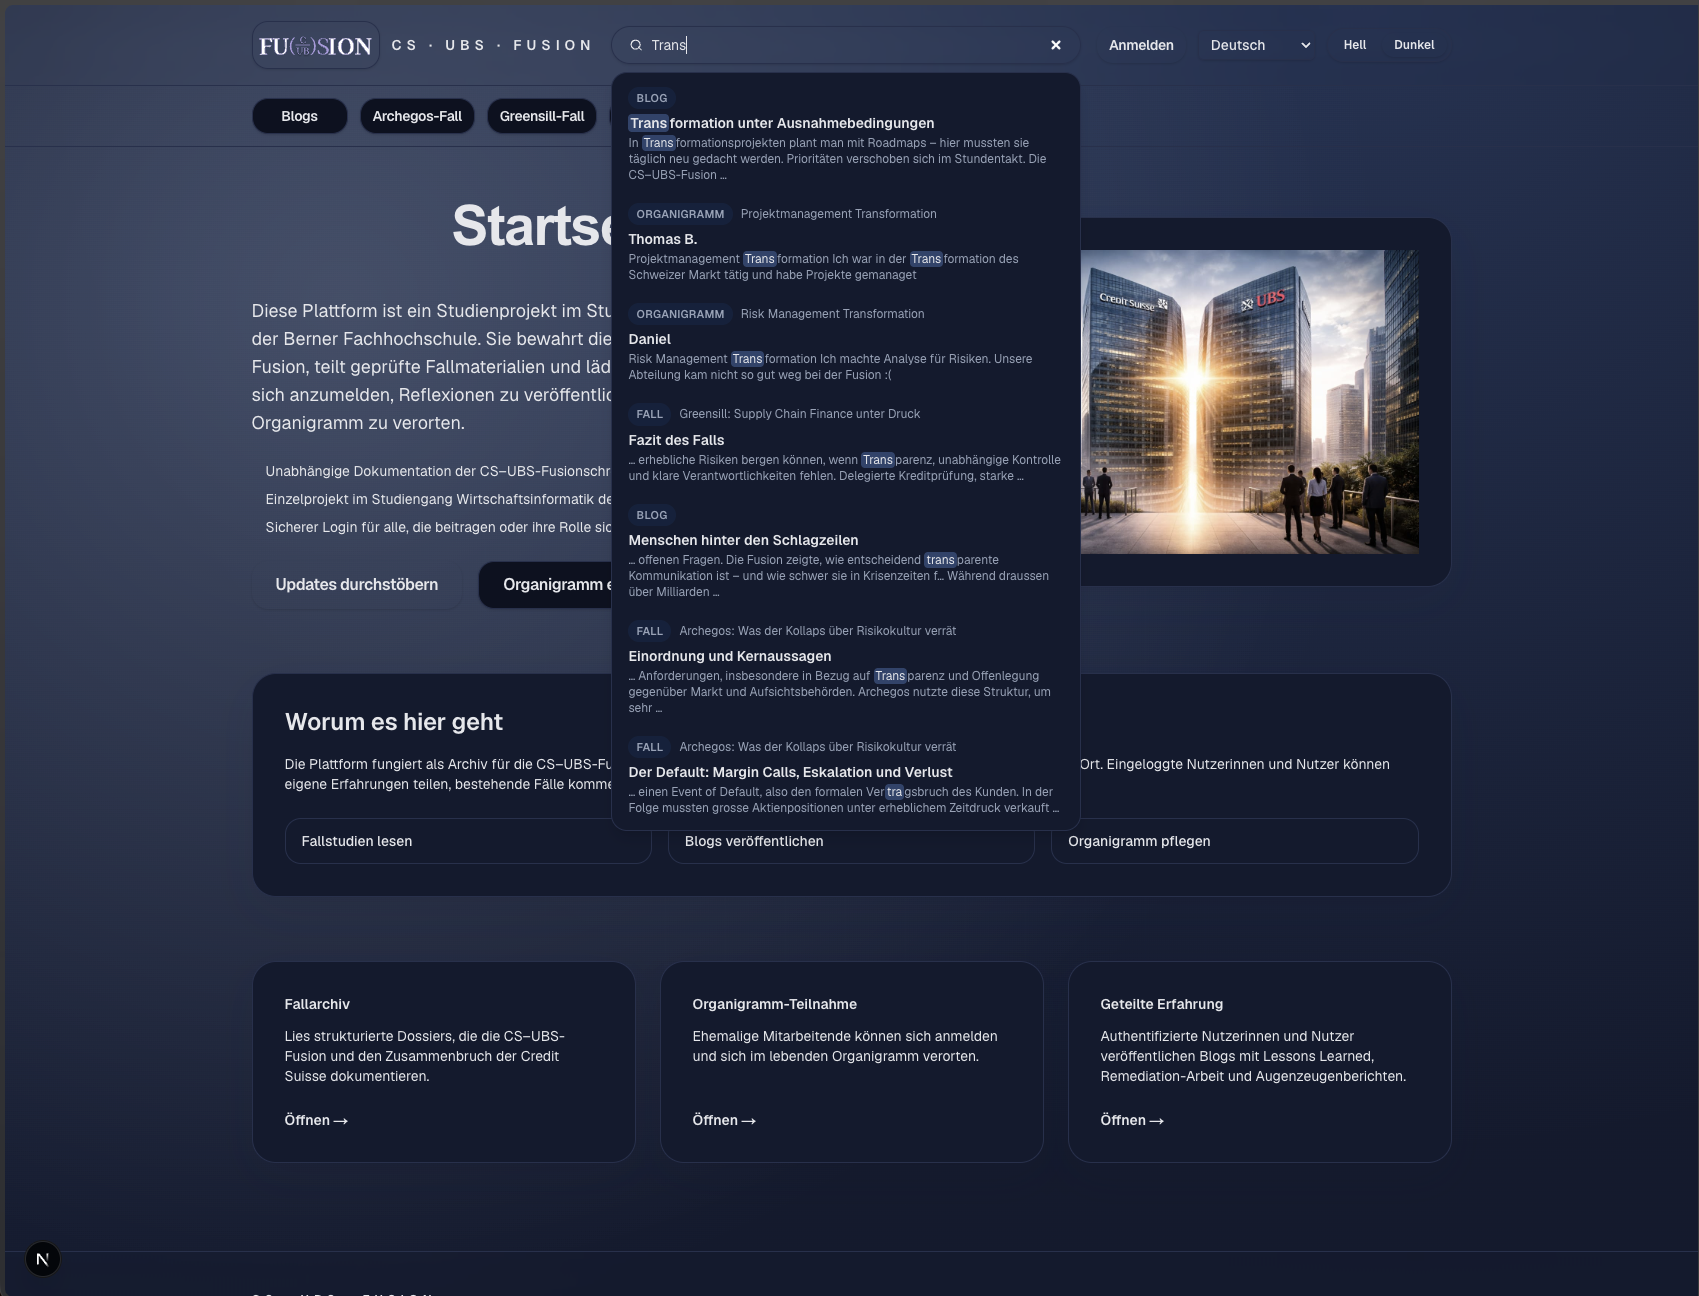
\includegraphics[width=0.85\textwidth]{screenshot_suche_trans.png}
  \caption{Suche nach „Trans“: Treffer aus Blog, Organigramm und Fällen}
  \label{fig:suche-trans}
\end{figure}

\begin{figure}[htbp]
  \centering
  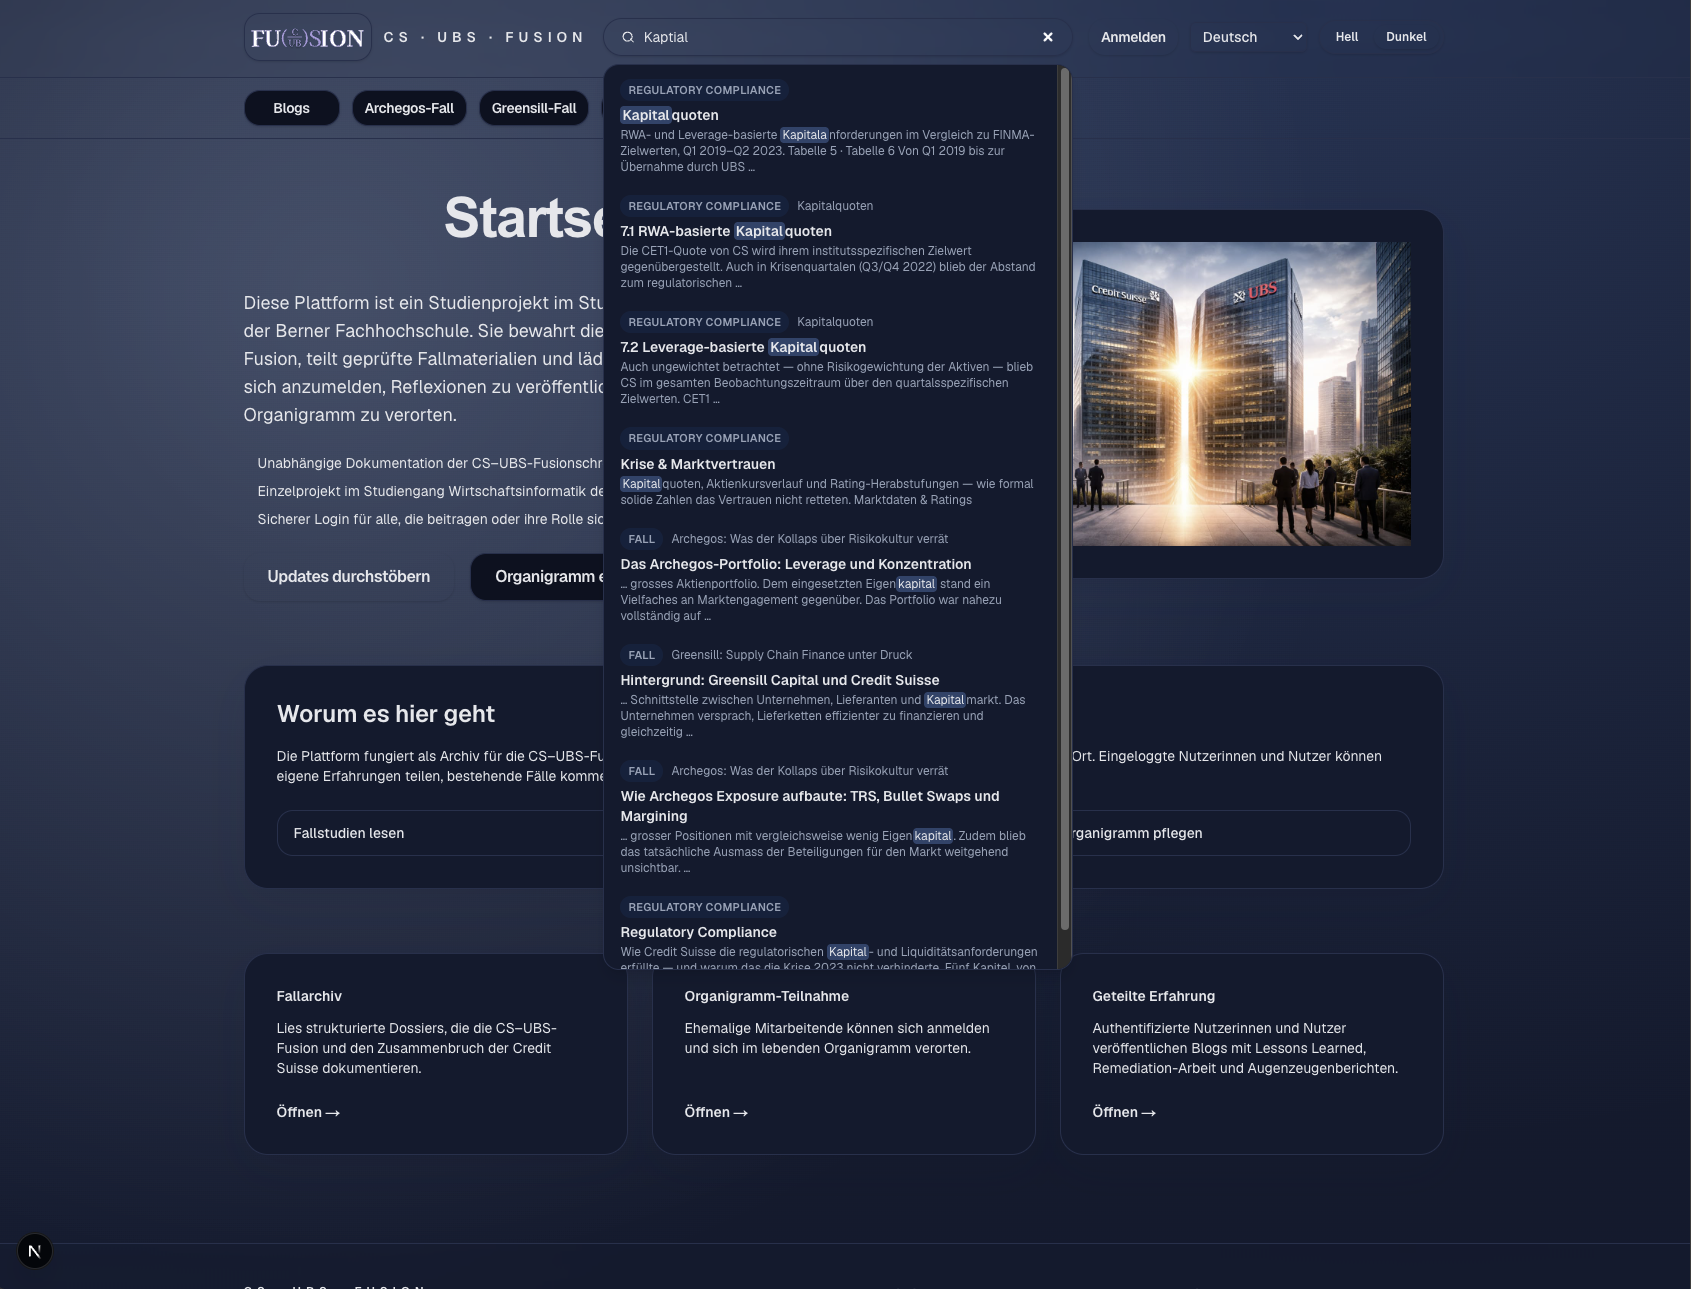
\includegraphics[width=0.85\textwidth]{screenshot_suche_kapital.png}
  \caption{Suche nach „Kaptial“ (Tippfehler): Treffer zu „Kapital“}
  \label{fig:suche-kapital}
\end{figure}

\subsection{Selbstreflexion}

\textbf{Was hat gut funktioniert}\par
Das Provider-Muster hat sich bewährt: Der Bereich Regulatory Compliance kam später dazu, ohne dass Route, Bewertung der Treffer oder Frontend geändert werden mussten. Damit ist die Anforderung der Wartbarkeit belegt. Gut war auch, dass ich Aufgabenliste und Testplan vor der Umsetzung festgelegt habe. Der Plan half mir, selbst nochmals besser darüber nachzudenken, und gab mir ein klareres Bild davon, was noch offen ist und wie es implementiert wird. Fuse.js im Speicher deckt alle Bereiche ab und braucht keine zusätzliche Infrastruktur.

\textbf{Wo musste nachgebessert werden}\par
Die Zusammenarbeit mit der KI lief sehr gut, weil ich schon Erfahrung mit dieser Arbeitsweise hatte. Es gab immer wieder kleine Verbesserungen, die sich aber mit weiterem Prompting oder einer kurzen Recherche im Web schnell beheben liessen. Konkret:
\begin{itemize}[nosep]
  \item Das Dokumentenmodell habe ich während der Umsetzung angepasst (\texttt{body} statt \texttt{snippet}, neues Feld \texttt{context}), weil die Treffer-Positionen sonst nicht zum gekürzten Text passten.
  \item HTML-Absätze klebten zusammen, und die Fall-Abschnitte füllten die Trefferliste fast ganz. Daraus entstand die Regel „höchstens 4 Treffer je Bereich“.
  \item Beim Deep-Link ins Organigramm brauchte es einen Zwischenspeicher, weil das Diagramm dynamisch nachgeladen wird. Der Parameter wird nach dem Öffnen aus der URL entfernt.
\end{itemize}

\textbf{Bestehende Fehler im Projekt}\par
Beim Testen bin ich auf zwei Fehler gestossen, die nicht von der Suche stammen: Die Farb-Utilities von Tailwind greifen projektweit nicht (Tailwind 4 mit Konfiguration im Stil von Tailwind 3), weshalb das Dropdown zunächst durchsichtig war. Ich habe das mit \texttt{hsl(var(--token))} umgangen. Ausserdem ist die Organigramm-Detailansicht wegen eines CSS-Transforms im Wrapper kein echtes Vollbild. Beides habe ich bewusst nicht behoben, weil es nicht zum Auftrag gehörte, und als eigene Arbeitspakete dokumentiert.

\textbf{Was ich gelernt habe}\par
Ein guter Prompt lohnt sich. Er sollte klären: Was ist der Stand jetzt, was will ich am Ende haben, soll die KI selbständig entscheiden oder nachfragen, und weiss ich schon etwas Spezifisches darüber, wie ich es umgesetzt haben möchte.

\textbf{Was ich nächstes Mal anders machen würde}\par
Ich würde vorab prüfen, ob Lint und Typecheck im Projekt laufen, denn \texttt{npm run lint} meldet wegen des Ordners \texttt{.claude} 18\,288 Probleme, obwohl der App-Code sauber ist. Dieser Ordner gehört in die ESLint-Ignorierliste. Ein Browser-Testläufer würde die manuellen Oberflächentests (Tastatur, Sprachwechsel) ersetzen.

% ------------------------------------------------------------
% 5 Aufgabe 3
% ------------------------------------------------------------
\section{Aufgabe 3: Themenbereich Regulatory Compliance}

\subsection{Auftrag und Mockups}
Besucher der Plattform sollen nachvollziehen können, dass die Credit Suisse trotz durchgehender Einhaltung der regulatorischen Kapitalanforderungen in eine existenzbedrohende Krise geriet. Dafür entsteht ein neuer Themenbereich „Regulatory Compliance“ mit eigener Navigation und fünf Unterseiten. Nur die erste Unterseite (Kapitalquoten) wird inhaltlich gefüllt, die übrigen vier bleiben als Platzhalter bestehen, damit die Struktur vollständig sichtbar ist.

Der Auftrag besteht aus vier Teilaufgaben:
\begin{enumerate}[nosep]
  \item \textbf{Navigation:} \texttt{navItems} in \texttt{navbar.tsx} um „Regulatory Compliance“ ergänzen. Auf \texttt{/regulatory-compliance/\allowbreak *} erscheint eine zweite Pill-Reihe mit den fünf Themen im bestehenden Pill-Stil, ohne neues Dropdown-Widget.
  \item \textbf{Übersichtsseite:} \texttt{/regulatory-compliance} mit fünf Karten (Titel, Kurzbeschreibung, Pfeil-Icon), die auf die Unterseiten verlinken.
  \item \textbf{Platzhalterseiten:} Alle fünf Routen anlegen, vier davon nur mit Titel und „Inhalt folgt“.
  \item \textbf{Kapitel-7-Seite mit Recharts:} Tabelle 5 und 6 als HTML-Tabelle, ein Recharts-Liniendiagramm (Ist vs. Zielwert), Key-Takeaways-Box und Quellenangabe.
\end{enumerate}

Der vollständige Auftragstext steht im Anhang~\ref{app:auftrag}. Dem Auftrag lagen drei Mockups bei (Abbildungen~\ref{fig:mock-nav} bis~\ref{fig:mock-kap7}), die als Vorlage für die Umsetzung dienten.

\begin{figure}[htbp]
  \centering
  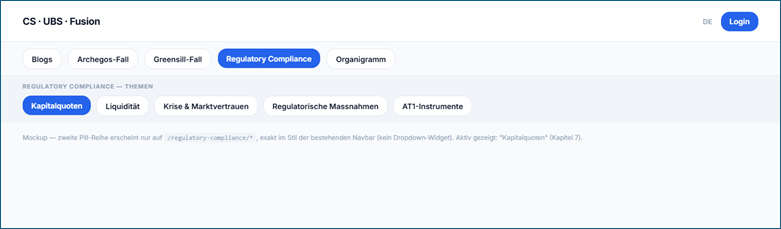
\includegraphics[width=0.9\textwidth]{mockup_navigation.png}
  \caption{Mockup Navigation: zweite Pill-Reihe unter \texttt{/regulatory-compliance/\allowbreak *}}
  \label{fig:mock-nav}
\end{figure}

\begin{figure}[htbp]
  \centering
  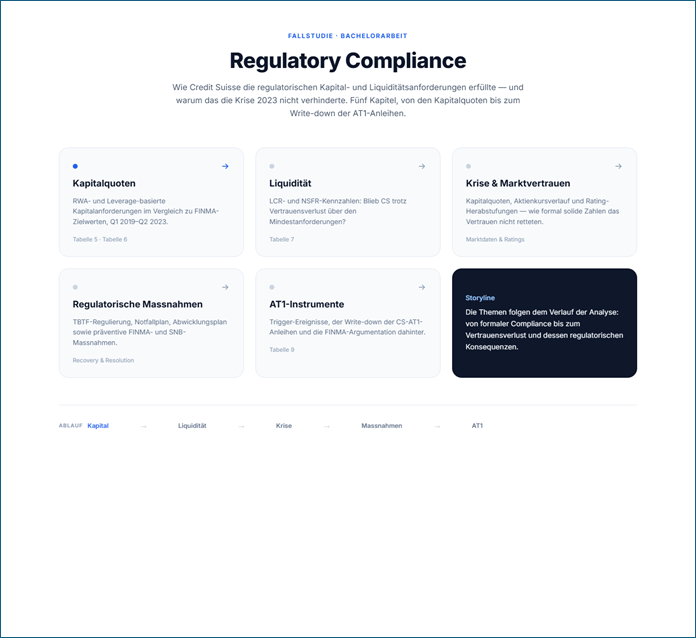
\includegraphics[width=0.75\textwidth]{mockup_uebersicht.png}
  \caption{Mockup Übersichtsseite mit fünf Karten und Storyline}
  \label{fig:mock-uebersicht}
\end{figure}

\begin{figure}[htbp]
  \centering
  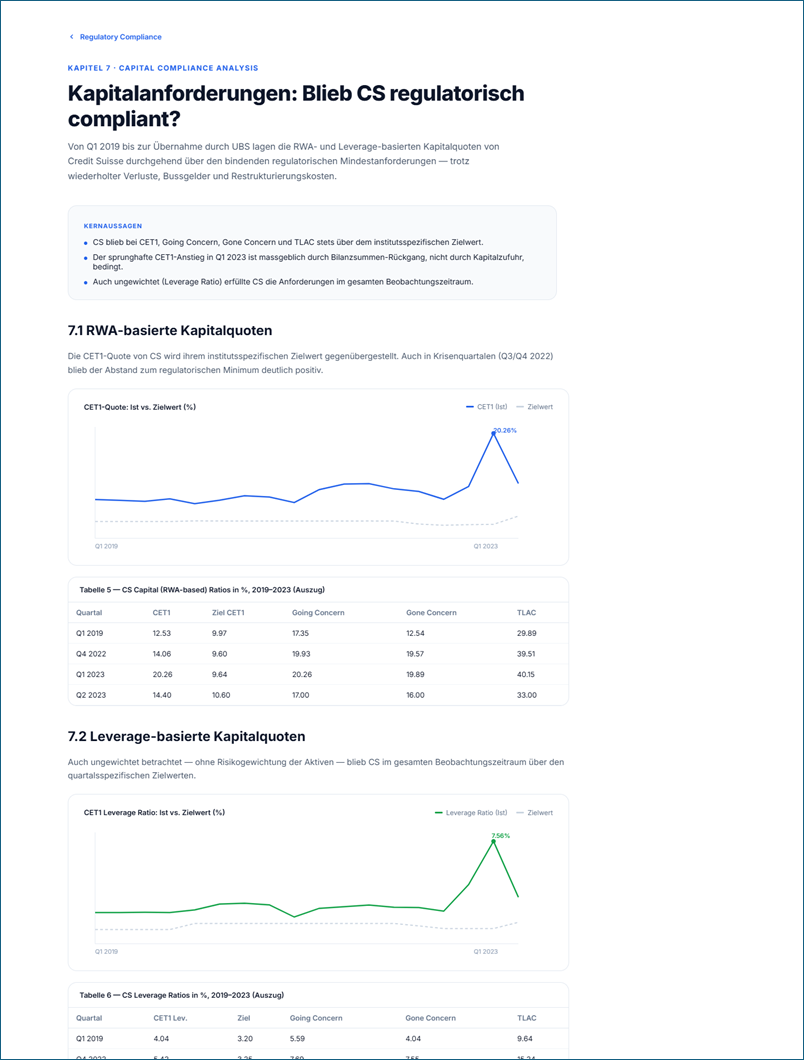
\includegraphics[width=0.7\textwidth]{mockup_kapitel7.png}
  \caption{Mockup Kapitel 7: Kapitalquoten mit Diagrammen und Tabellen}
  \label{fig:mock-kap7}
\end{figure}

\subsection{Geklärte Fragen und Entscheidungen}
Bevor der Umsetzungsplan entstand, habe ich fünf Fragen geklärt, die weder der Auftrag noch die Mockups beantworteten. Jede Antwort legt eine Entscheidung im Plan fest.

\begin{center}
\small
\begin{longtable}{@{}>{\raggedright\arraybackslash}p{4.4cm} >{\raggedright\arraybackslash}p{3.6cm} >{\raggedright\arraybackslash}p{6.8cm}@{}}
\toprule
\textbf{Frage} & \textbf{Antwort} & \textbf{Entscheidung im Plan} \\
\midrule
\endhead
Woher stammen die vollständigen Daten für Tabelle 5 und 6? Das Mockup zeigt nur 4 Zeilen. & Nur den Auszug zeigen & Tabellen und Diagramme nutzen die 4 Quartale aus dem Mockup: Q1 2019, Q4 2022, Q1 2023, Q2 2023. \\
\midrule
Welche Sprachen soll der neue Inhalt haben? & Alle 5 über die Sprachdateien & Alle neuen Schlüssel kommen in alle 5 Dateien \texttt{messages/*.json}. \\
\midrule
Welche URL-Slugs sollen die Unterseiten haben? & Bestehende Lösung prüfen & Die Seite nutzt für alle Sprachen einen englischen Slug, weil \texttt{i18n/routing.ts} keine \texttt{pathnames} kennt. \\
\midrule
Sollen die neuen Seiten in Sitemap und Suche? & Sitemap und Suche & Neue Pfade in \texttt{app/sitemap.ts} und ein neuer Suchprovider. \\
\midrule
In Tabelle 6 ist nur Q1 2019 vollständig lesbar. Können die Werte geliefert werden? & Die 3 sichtbaren Werte verwenden & Q1 2019 vollständig, Q4 2022 abgelesen, Q1 2023 nur CET1-Leverage (7.56). Alle anderen Zellen bleiben leer und zeigen „–“. \\
\bottomrule
\end{longtable}
\end{center}

Daraus ergaben sich diese Routen:
\begin{center}
\footnotesize
\begin{tabular}{@{}>{\raggedright\arraybackslash}p{3.5cm} >{\raggedright\arraybackslash}p{7.3cm} >{\raggedright\arraybackslash}p{3.6cm}@{}}
\toprule
\textbf{Thema} & \textbf{Route} & \textbf{Status} \\
\midrule
Übersicht & \texttt{/regulatory-compliance} & Inhalt \\
Kapitalquoten (Kapitel 7) & \texttt{/regulatory-compliance/\allowbreak capital-ratios} & Inhalt (Tabellen, Diagramme) \\
Liquidität & \texttt{/regulatory-compliance/\allowbreak liquidity} & Platzhalter \\
Krise \& Marktvertrauen & \texttt{/regulatory-compliance/\allowbreak crisis-market-confidence} & Platzhalter \\
Regulatorische Massnahmen & \texttt{/regulatory-compliance/\allowbreak regulatory-measures} & Platzhalter \\
AT1-Instrumente & \texttt{/regulatory-compliance/\allowbreak at1-instruments} & Platzhalter \\
\bottomrule
\end{tabular}
\end{center}

\subsection{Umsetzung}
\begin{itemize}[nosep]
  \item \textbf{Navigation:} \texttt{navbar.tsx} enthält den neuen Eintrag „Regulatory Compliance“. Unter \texttt{/regulatory-compliance/\allowbreak *} erscheint eine zweite Pill-Reihe mit den fünf Themen im bestehenden Pill-Stil, ohne neues Dropdown-Widget.
  \item \textbf{Übersichtsseite:} Fünf Karten mit Titel, Kurzbeschreibung und Pfeil-Icon, eine Storyline-Kachel und eine Ablauf-Leiste (Kapital, Liquidität, Krise, Massnahmen, AT1).
  \item \textbf{Platzhalterseiten:} Eine gemeinsame dynamische Route \texttt{[topic]} für die vier noch leeren Themen mit Titel und „Inhalt folgt“.
  \item \textbf{Kapitel 7:} Die Seite \texttt{capital-ratios} zeigt Key-Takeaways, je ein Recharts-Liniendiagramm (Ist gegen Zielwert) und die Tabellen 5 und 6 als HTML-Tabellen. Die Komponenten \texttt{RatioChart} und \texttt{RatioTable} sind wiederverwendbar, die Zahlen liegen sprachunabhängig in \texttt{lib/regulatoryCompliance/capitalRatios.ts}. Die Abschnitte haben die Sprungmarken \texttt{\#rwa} und \texttt{\#leverage}. Auf eine eigene Quellenangabe wurde verzichtet, weil die Daten und Mockups vom Auftraggeber stammen.
  \item \textbf{Übersetzungen:} Alle Texte stehen in den fünf Sprachdateien. Die Texte für Französisch, Spanisch und Italienisch sind Beispielinhalte beziehungsweise sinngemässe Übersetzungen und wurden nicht fachlich geprüft.
  \item \textbf{Sitemap und Suche:} Die sechs neuen Pfade stehen in \texttt{app/sitemap.ts}. Ein neuer Suchprovider \texttt{regulatoryCompliance} macht Übersicht, Themen und die beiden Kapitel-7-Abschnitte auffindbar (siehe Abschnitt~4.3).
  \item \textbf{Abhängigkeit:} Neu ist \texttt{recharts} in Version \texttt{\^{}3.10.1}.
\end{itemize}

\subsection{Vorgehen mit parallelen Agents}
Den Umsetzungsplan hat Claude Code aus dem Auftrag und den Mockups erstellt. Er ist so aufgebaut, dass mehrere Agents gleichzeitig daran arbeiten können. Die Umsetzung lief in drei Phasen:
\begin{enumerate}[nosep]
  \item \textbf{Phase 1, Foundation} (Branch \texttt{rc/foundation}): Ein Agent legt die gemeinsame Basis an, also gemeinsame Konfiguration, Recharts und alle Übersetzungsschlüssel.
  \item \textbf{Phase 2, Tracks A bis E} (parallel): Fünf Agents arbeiten gleichzeitig, jeder in einem eigenen Git-Worktree und auf einem eigenen Branch und nur an seinen eigenen Dateien. Track A: Navigation (\texttt{rc/nav}). Track B: Übersicht und Platzhalter (\texttt{rc/overview}). Track C: Kapitel 7 (\texttt{rc/capital}). Track D: Sitemap und Suche (\texttt{rc/search}). Track E: Übersetzungen (\texttt{rc/i18n}).
  \item \textbf{Phase 3, Integration} (Branch \texttt{rc/integration}): Ein Agent führt die Branches zusammen und führt die Prüfungen durch. Danach wurde \texttt{rc/integration} nach \texttt{main} gemerged.
\end{enumerate}
Die Aufteilung nach Dateien verhindert Merge-Konflikte. Der Plan liegt im Repository unter \texttt{todo/plan.md}.

\subsection{Test und Review}
Für Aufgabe 3 gibt es 13 manuelle Testfälle (TC1 bis TC13) in \texttt{todo/testcases.md}. Sie decken Hauptnavigation, zweite Pill-Reihe, Übersichtsseite, Links, Platzhalter, Aufbau, Diagramme und Tabellen von Kapitel 7, Anker und Suche, Sprachen, Dark Mode, Mobile-Ansicht sowie Sitemap und Direktaufrufe ab. Jeder Testfall hat Schritte und ein erwartetes Ergebnis. Die Suche ist zusätzlich durch drei automatisierte Tests abgedeckt (T21 bis T23): Suche nach „CET1“ und „Kapitalquoten“ führt auf die Kapitalquoten-Seite, und der Abschnitt 7.1 verlinkt auf die Sprungmarke \texttt{\#rwa}.

Zusätzlich liegt ein Review-Dokument mit Befunden zur Umsetzung vor (\texttt{todo/\allowbreak review-\allowbreak regulatory-\allowbreak compliance.md}). Beim Gegenprüfen gegen den Code trafen zwei der als kritisch bezeichneten Befunde nicht zu: Der Export \texttt{RC\_\allowbreak CAPITAL\_\allowbreak RATIOS\_\allowbreak ANCHORS} existiert in \texttt{lib/\allowbreak regulatoryCompliance.ts}, und die Testkonstanten \texttt{rcTerm} und \texttt{rcTopic} sind definiert. Ein solches Review muss deshalb selbst überprüft werden.

\subsection{Ergebnis}
Der neue Themenbereich ist in die Applikation integriert. Abbildung~\ref{fig:rc-uebersicht} zeigt die Übersichtsseite mit der aktiven Haupt-Pill „Regulatory Compliance“, der zweiten Pill-Reihe mit den fünf Themen, den fünf Karten, der Storyline-Kachel und der Ablauf-Leiste. Die Kapitel-7-Seite (Abbildungen~\ref{fig:rc-kap7-oben} und~\ref{fig:rc-kap7-tabellen}) enthält die Kernaussagen, das CET1-Liniendiagramm mit Ist- und Zielwert sowie Tabelle 5 als HTML-Tabelle. Die Platzhalterseiten zeigen Titel, Kurzbeschreibung und „Inhalt folgt“ (Abbildung~\ref{fig:rc-platzhalter}).

\begin{figure}[htbp]
  \centering
  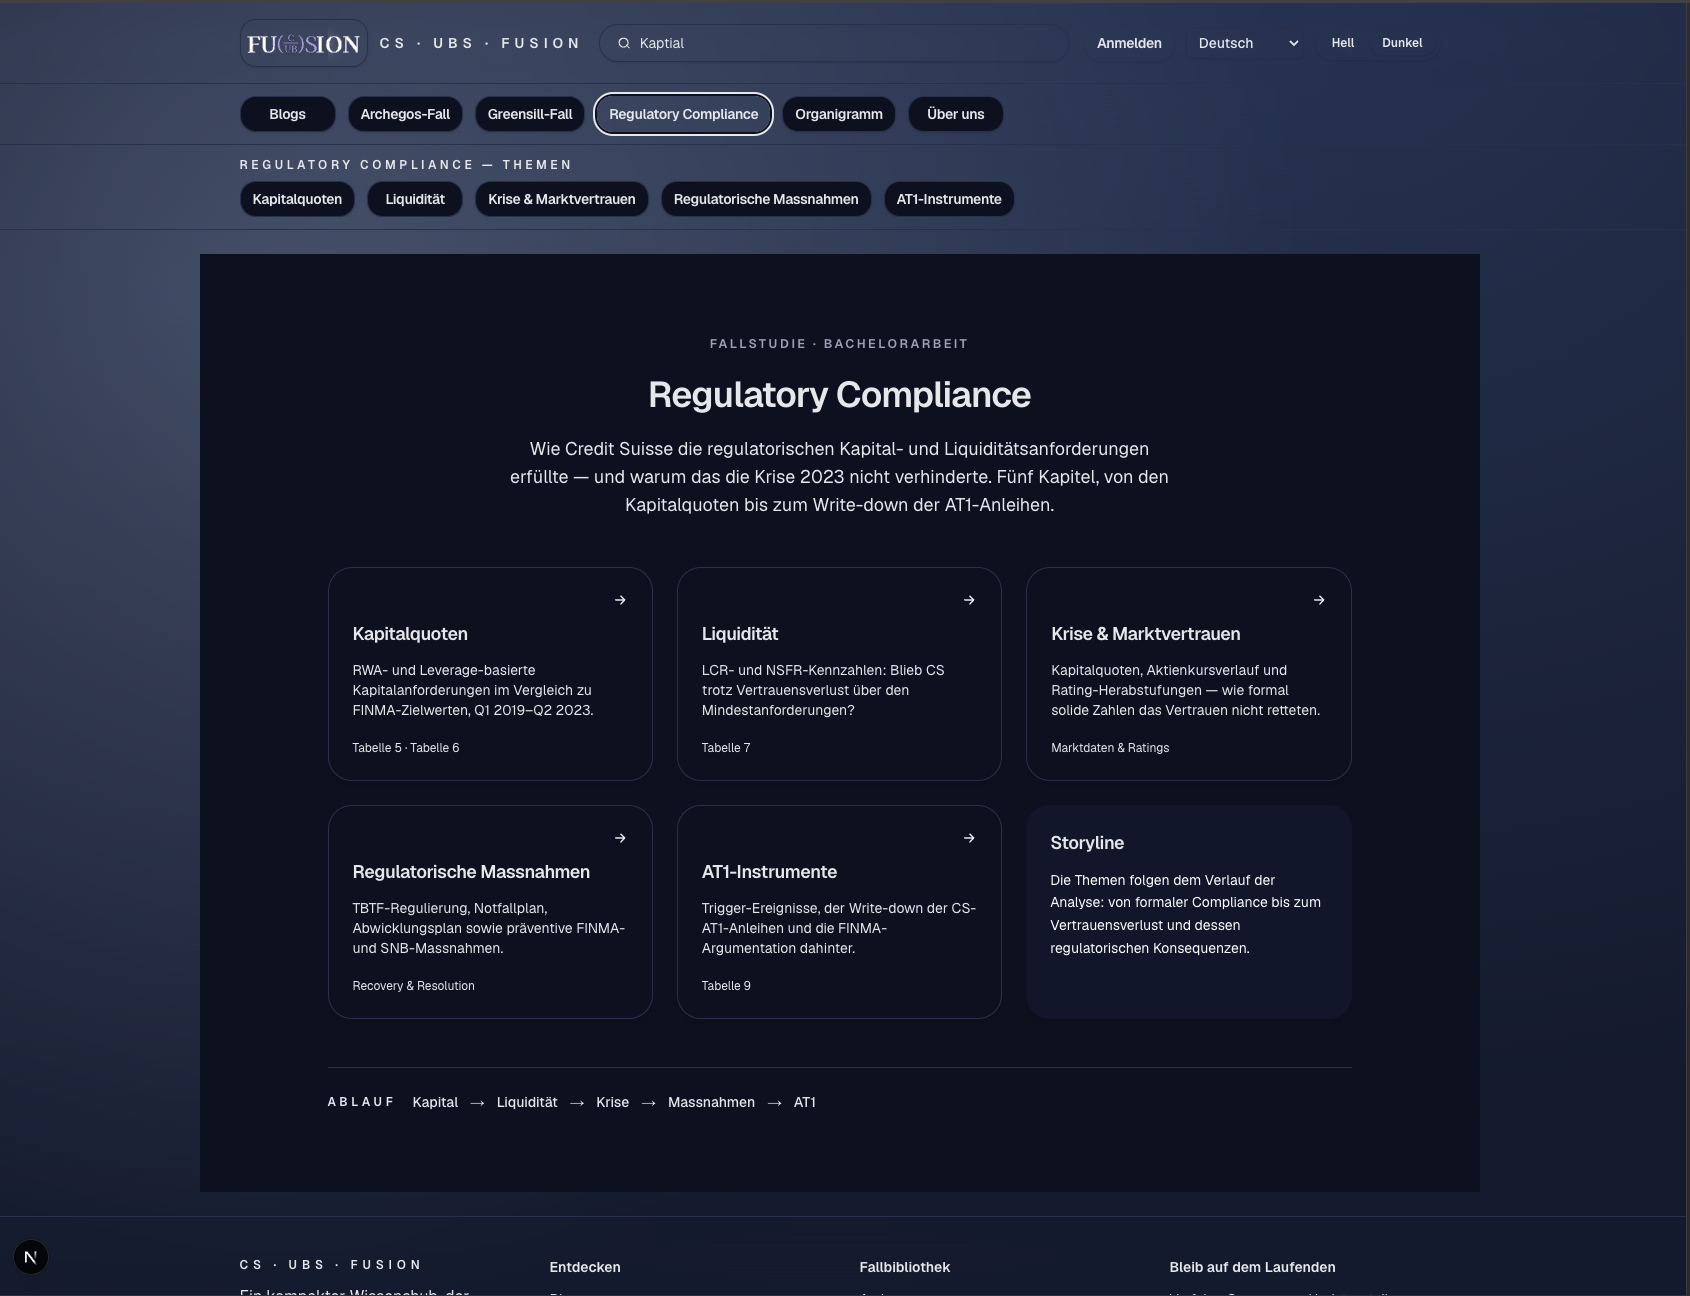
\includegraphics[width=0.9\textwidth]{screenshot_rc_uebersicht.png}
  \caption{Übersichtsseite Regulatory Compliance mit zweiter Pill-Reihe, fünf Karten, Storyline und Ablauf-Leiste}
  \label{fig:rc-uebersicht}
\end{figure}

\begin{figure}[htbp]
  \centering
  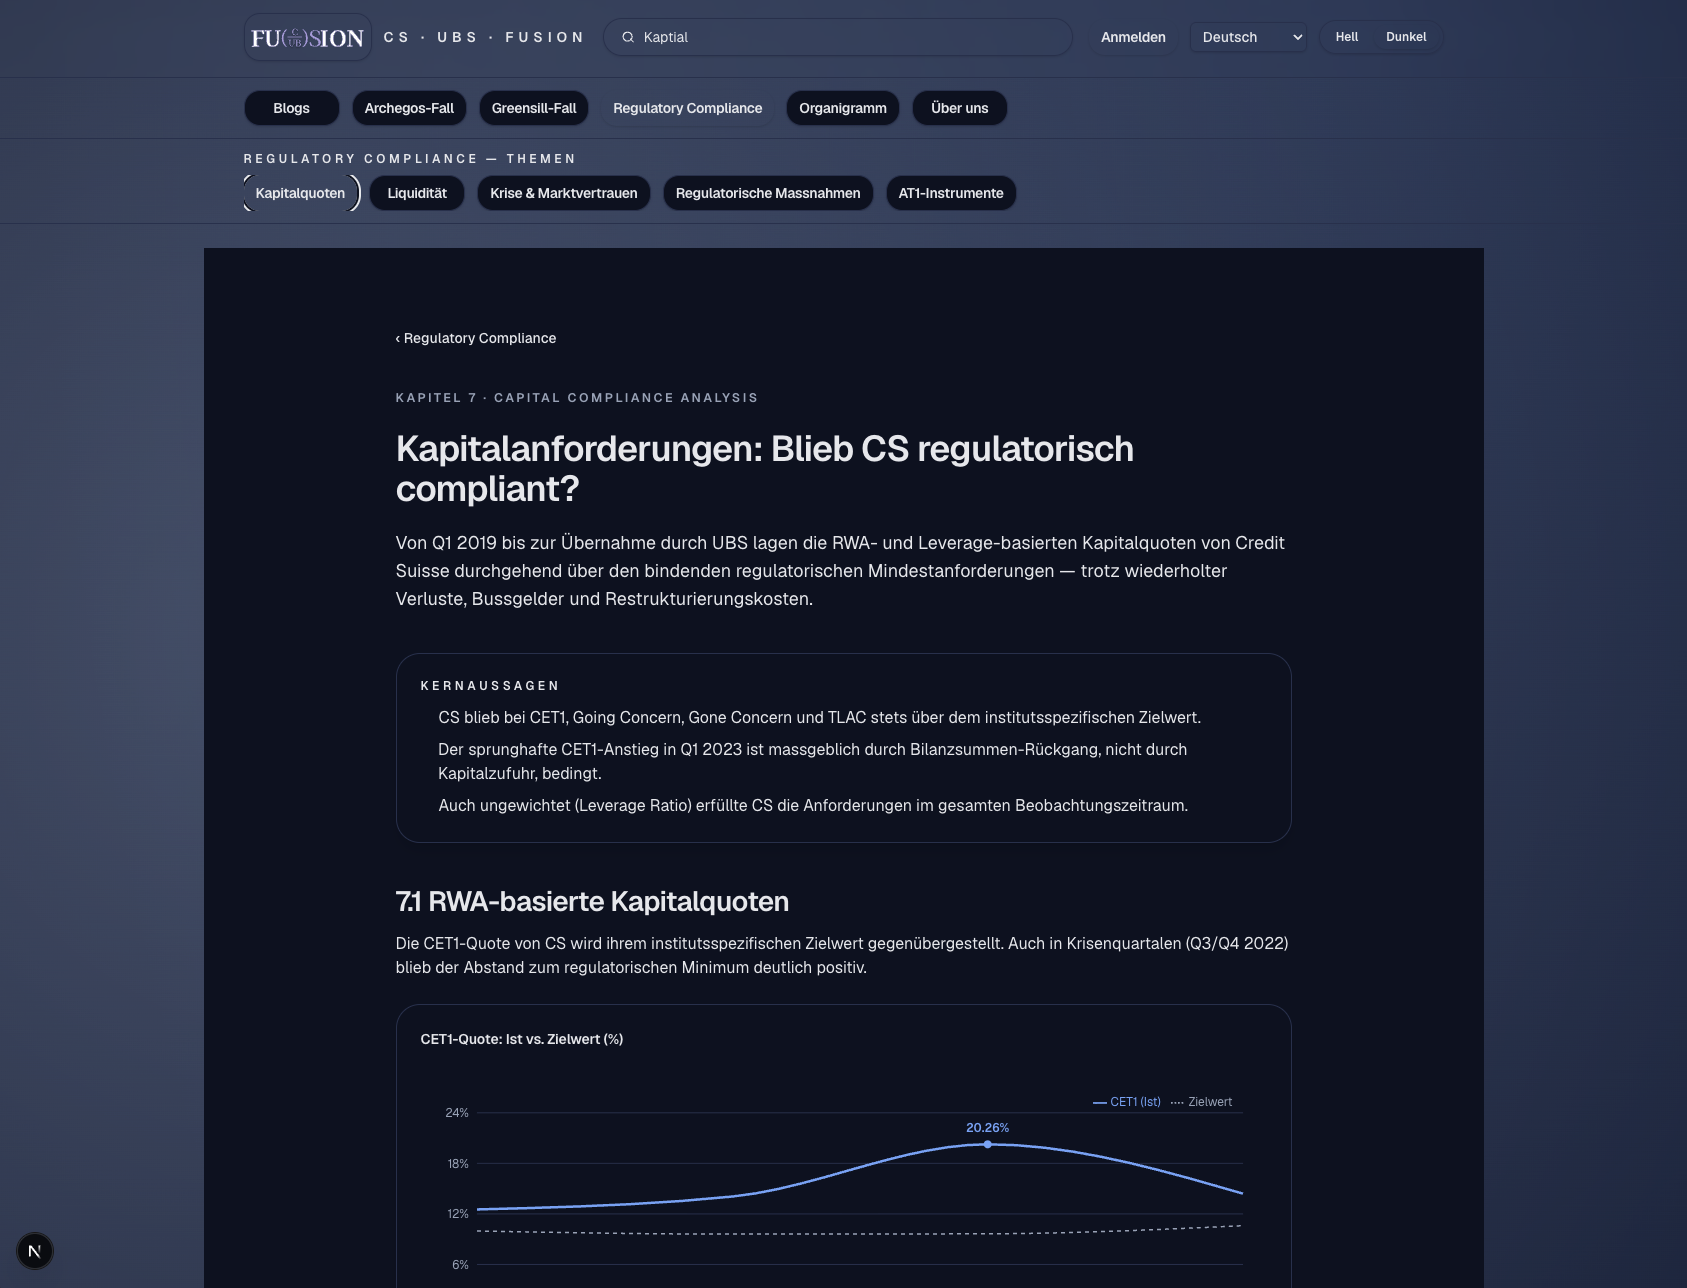
\includegraphics[width=0.9\textwidth]{screenshot_rc_kapitel7_oben.png}
  \caption{Kapitel 7: Titel, Kernaussagen und CET1-Diagramm (Ist gegen Zielwert)}
  \label{fig:rc-kap7-oben}
\end{figure}

\begin{figure}[htbp]
  \centering
  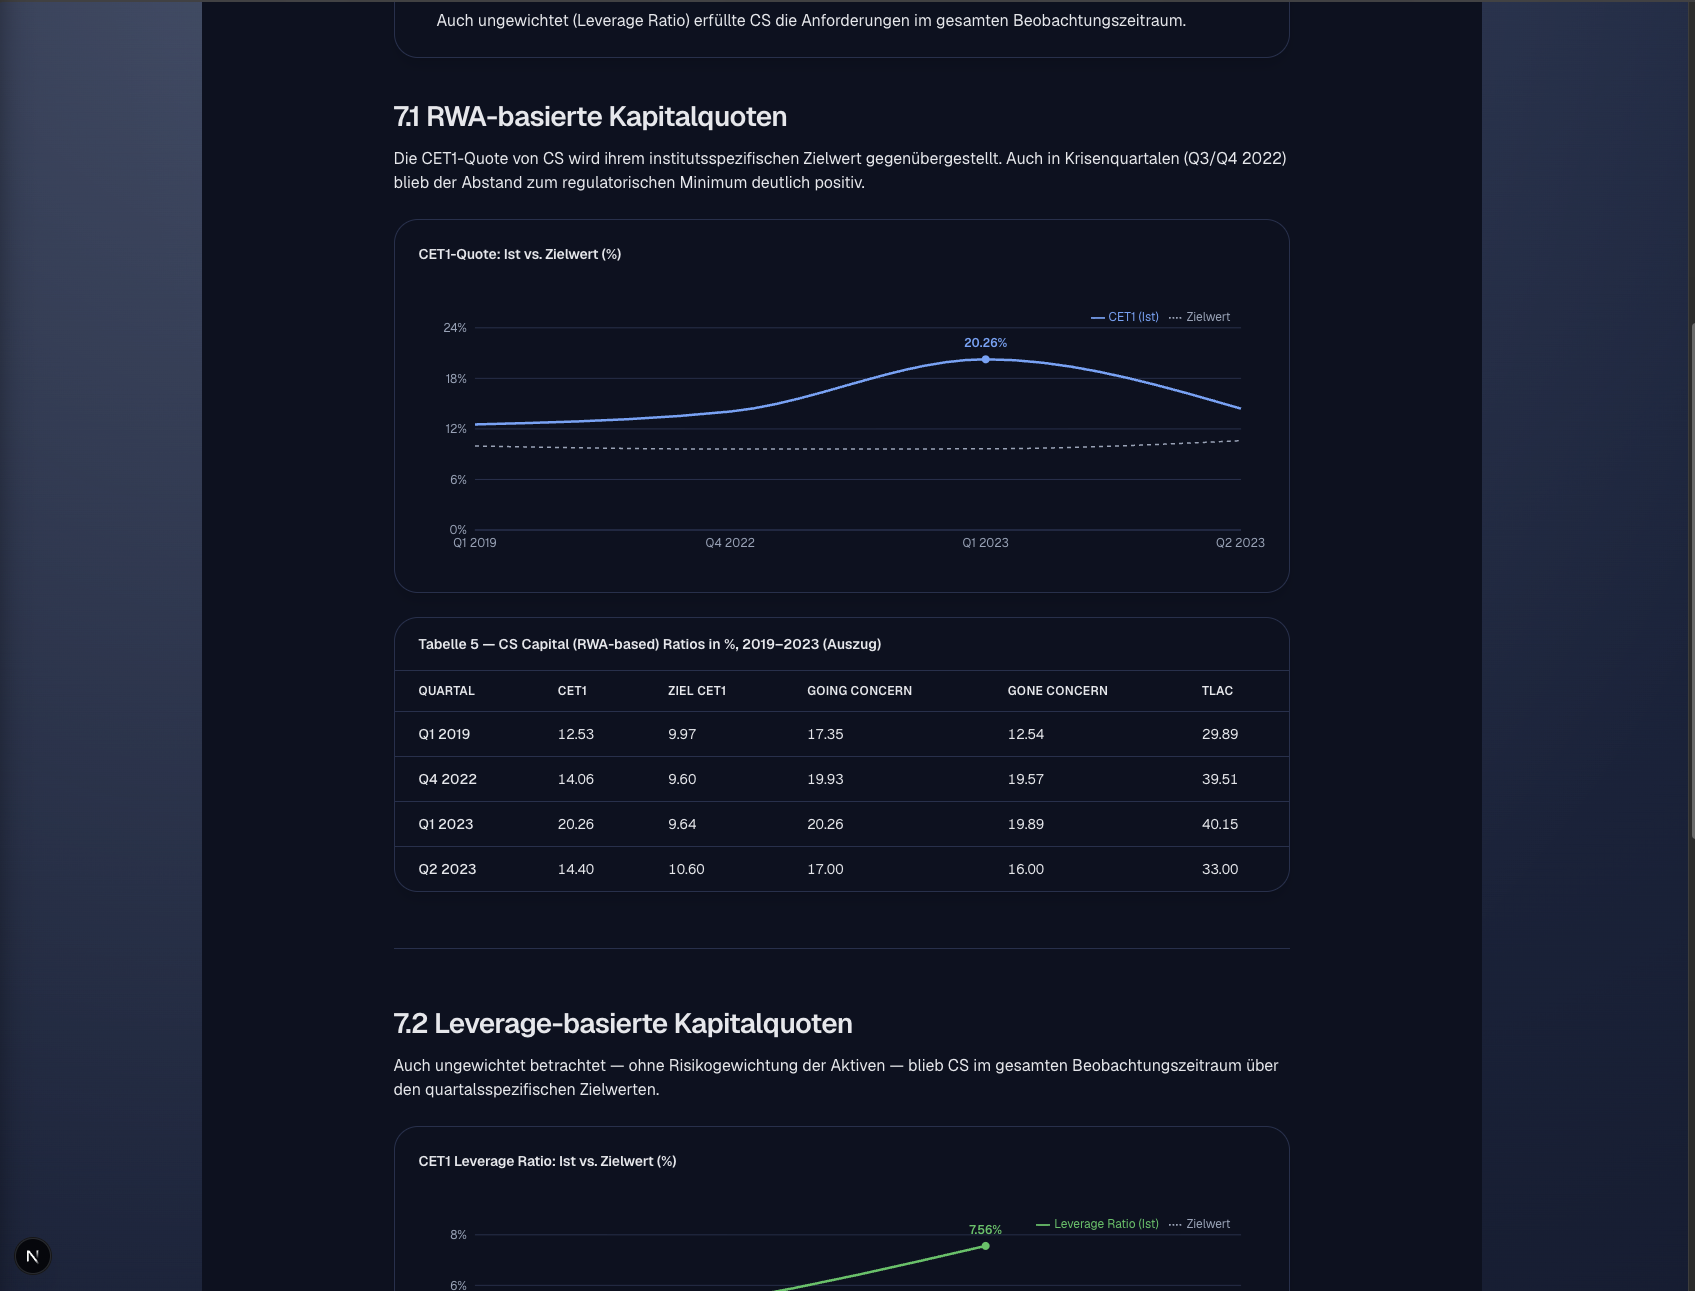
\includegraphics[width=0.9\textwidth]{screenshot_rc_kapitel7_tabellen.png}
  \caption{Kapitel 7: CET1-Diagramm und Tabelle 5 (RWA-basierte Kapitalquoten, Auszug)}
  \label{fig:rc-kap7-tabellen}
\end{figure}

\begin{figure}[htbp]
  \centering
  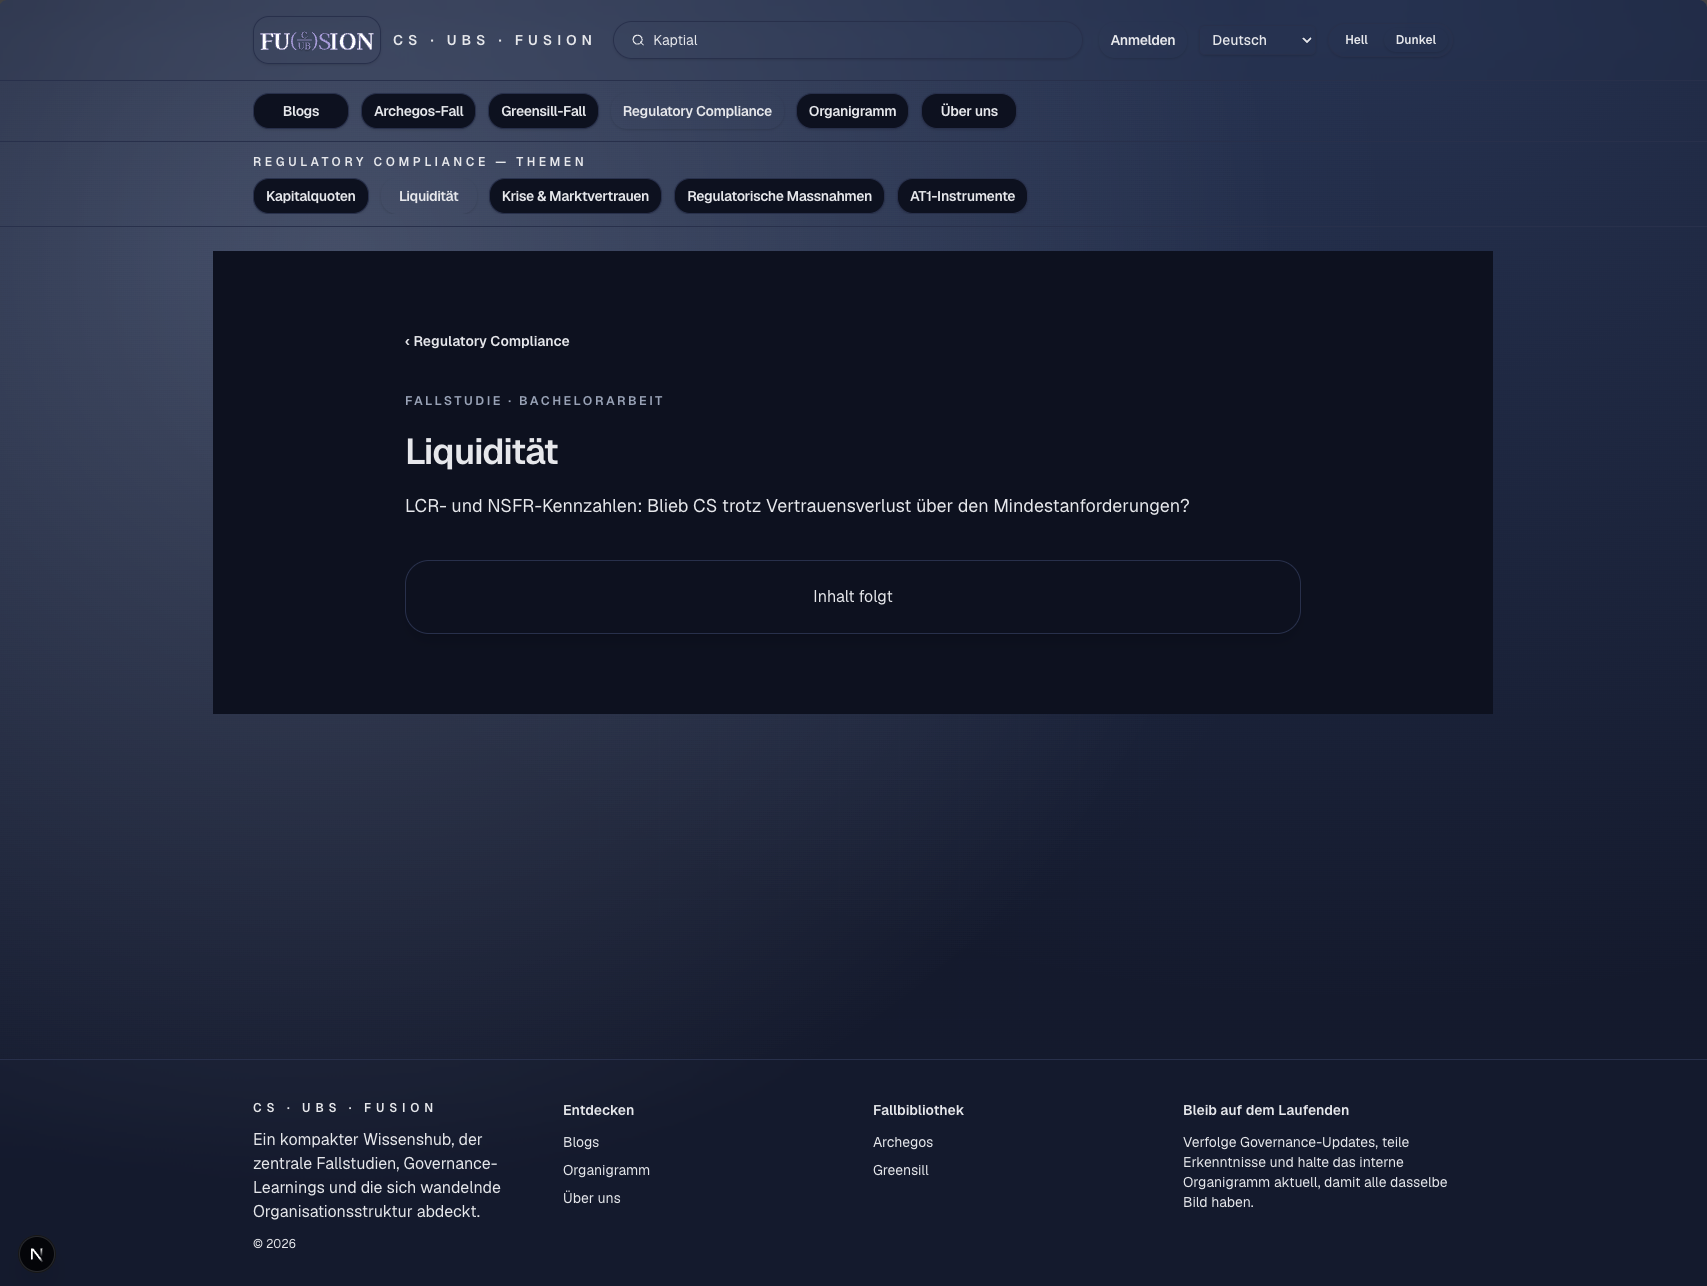
\includegraphics[width=0.9\textwidth]{screenshot_rc_platzhalter.png}
  \caption{Platzhalterseite „Liquidität“ mit dem Hinweis „Inhalt folgt“}
  \label{fig:rc-platzhalter}
\end{figure}

\subsection{Selbstreflexion}
Die Arbeit lief sehr gut. Die parallele Arbeit in eigenen Branches und Worktrees hat sie übersichtlich gehalten, und die Aufteilung nach Dateien vermied weitgehend Konflikte. Es gab nur kleine Probleme beim Zusammenführen der Branches, die sich ebenfalls durch Agents lösen liessen. Der Verbrauch an Token war etwas höher als üblich, dafür war die Umsetzung insgesamt sehr schnell. Der Plan mit festgelegten Entscheidungen half mir, offene Punkte früh zu sehen. Als Datengrundlage dienten die Unterlagen des Auftraggebers. Offen blieb die fachliche Prüfung der Übersetzungen für Französisch, Spanisch und Italienisch, die als Beispielinhalte angelegt sind.

% ------------------------------------------------------------
% 6 Kritische Gesamtreflexion
% ------------------------------------------------------------
\section{Kritische Gesamtreflexion}

\subsection{Lessons Learned über alle drei Aufgaben}
\begin{itemize}[nosep]
  \item \textbf{Ein guter Prompt lohnt sich.} Er klärt, was der Stand jetzt ist, was am Ende herauskommen soll, ob die KI selbständig entscheiden oder nachfragen soll und ob ich schon etwas Spezifisches über die gewünschte Umsetzung weiss. Der Prompt-Vergleich in Aufgabe 1 zeigte, dass in meinen Rohprompts immer wieder der vollständige Ist-Zustand und die Nebenabhängigkeiten fehlten.
  \item \textbf{Ein Plan vor der Umsetzung hilft.} Er verschafft einen besseren Überblick darüber, was offen ist und wie es umgesetzt wird, und macht die Arbeit überprüfbar.
  \item \textbf{Offizielle Werkzeuge zuerst.} Die Codemods übernahmen den grössten Teil des Next.js-Updates zuverlässig.
  \item \textbf{Unabhängige Aufgaben lassen sich parallelisieren,} wenn sie nach Dateien getrennt sind (Aufgabe 3).
  \item \textbf{Vorhandene Fehler im Projekt tauchen beim Testen auf.} Hier waren das die Tailwind-Konfiguration und die Organigramm-Detailansicht.
\end{itemize}

\subsection{Wo KI geholfen hat und wo sie Fehler eingebracht hat}
Geholfen hat die KI vor allem bei der Planung und der Codierung (Claude Code), bei der Aufteilung in parallele Arbeitspakete und bei der Gegenprüfung des Codes durch weitere Modelle. Die Zusammenarbeit lief sehr gut, weil ich bereits Erfahrung mit dieser Arbeitsweise hatte. Fehler und Lücken gab es immer wieder in kleinem Mass, sie liessen sich aber mit weiterem Prompting oder einer kurzen Recherche schnell beheben.

Beispiele für Lücken und Fehler:
\begin{itemize}[nosep]
  \item Das vorgesehene Update auf Prisma 7 war nicht möglich, weil Prisma 7 MongoDB nicht unterstützt. Dieses Detail zeigte sich erst später, weil mein Rohprompt nicht gezielt nach der MongoDB-Kompatibilität fragte (Aufgabe 1).
  \item Nach dem Next.js-Update schlug der Produktions-Build zunächst fehl, und es waren manuelle Korrekturen nötig (Aufgabe 1).
  \item Das Dokumentenmodell der Suche musste während der Umsetzung angepasst werden, und HTML-Absätze klebten zusammen (Aufgabe 2).
  \item Ein Review-Dokument zu Aufgabe 3 enthielt Befunde, die im Code nicht zutrafen (fehlender Export, nicht definierte Testkonstanten). Das Review musste selbst überprüft werden.
\end{itemize}

\subsection{Was beim nächsten Mal anders gemacht würde}
\begin{itemize}[nosep]
  \item Prompts von Anfang an mit vollständigem Ist-Zustand, Nebenabhängigkeiten, Testkontext und Antwortformat schreiben.
  \item Vorab prüfen, ob Lint und Typecheck im Projekt laufen.
  \item Ein Test-Framework oder einen Browser-Testläufer einrichten, damit die manuellen Oberflächentests entfallen.
  \item Offene Rückfragen (zum Beispiel zu Datenquellen und abgelesenen Werten) früher klären, statt sie bis zum Schluss mitzuführen.
\end{itemize}

% ------------------------------------------------------------
% 7 Fazit
% ------------------------------------------------------------
\section{Fazit}
Die drei Aufgaben wurden umgesetzt. Die App läuft auf Next.js 16.3.2 und React 19.2.8, Prisma wurde mit 6.19 auf die für MongoDB empfohlene Version aktualisiert. Das bisher funktionslose Suchfeld durchsucht jetzt Fälle, Blogs und Organigramm in fünf Sprachen, mit Vorschlägen während der Eingabe, Hervorhebung, Tippfehlertoleranz und Tastaturbedienung. Der neue Themenbereich „Regulatory Compliance“ hat Navigation, Übersicht, Platzhalterseiten und eine Kapitel-7-Seite mit Diagrammen und Tabellen. Die wichtigste Erkenntnis ist, dass die Qualität der Ergebnisse bei der Arbeit mit KI stark von der Qualität der Prompts und der Planung abhängt und dass jedes Resultat überprüft werden muss. Einschränkungen bleiben: Kapitel 7 zeigt nur einen Auszug der Daten, vier der fünf Unterseiten sind Platzhalter, und es gibt weiterhin kein automatisiertes Testframework für die Oberfläche.

% ------------------------------------------------------------
% 8 Ausblick
% ------------------------------------------------------------
\section{Ausblick}

\subsection{Verbesserungspotenzial}
\begin{itemize}[nosep]
  \item Die Farb-Utilities von Tailwind reaktivieren, indem in \texttt{globals.css} eine \texttt{@config}-Direktive ergänzt wird. Das verändert allerdings das Erscheinungsbild vieler bestehender Seiten.
  \item Die Organigramm-Detailansicht zu einem echten Vollbild-Overlay machen (Ursache: CSS-Transform im Wrapper).
  \item Die Suche um eine eigene Ergebnisseite, Filter nach Bereich und einen vorberechneten Index erweitern, falls die Datenmenge stark wächst. Zudem sind die Blog-Tags aktuell nie befüllt und liefern keine Treffer.
  \item Ein Browser-Testläufer für die Oberflächentests und eine Prüfung der Barrierefreiheit mit Screenreader.
  \item Fall-Slugs an einer zentralen Stelle verwalten statt an vier Orten.
  \item Neue Übersetzungsschlüssel in i18nexus nachziehen, falls die Sprachdateien dort verwaltet werden.
\end{itemize}

\subsection{Nächste Schritte}
\begin{itemize}[nosep]
  \item Die vier Platzhalterseiten von Regulatory Compliance mit Inhalt füllen (Liquidität, Krise und Marktvertrauen, Regulatorische Massnahmen, AT1-Instrumente).
  \item Tabellen 5 und 6 mit der vollständigen Zeitreihe von Q1 2019 bis Q2 2023 ergänzen.
  \item Die Übersetzungen für Französisch, Spanisch und Italienisch fachlich prüfen.
\end{itemize}

% ------------------------------------------------------------
% 9 Deklaration
% ------------------------------------------------------------
\section{Deklaration}

\subsection{Wortzahl}
Die Länge des vorliegenden Textes ab Kapitel 1 bis vor diesen Abschnitt beträgt rund 4900 Wörter (gezählt mit \texttt{texcount}, ohne Anhänge). Diese Zahl muss nach den letzten Änderungen am Text noch einmal gezählt werden.

\subsection{Selbständigkeitserklärung}
Ich bestätige, die vorliegende Arbeit selbständig verfasst zu haben. Sämtliche Textstellen, die nicht von mir stammen, sind als Zitate gekennzeichnet und mit dem genauen Hinweis auf ihre Herkunft versehen.

\subsection{Deklaration des KI-Einsatzes}
Für diese Arbeit wurden folgende KI-Werkzeuge eingesetzt (Details siehe Abschnitt~2.2):
\begin{itemize}[nosep]
  \item \textbf{Claude Code (CLI):} Hauptwerkzeug für die Planung und die Codierung des Projekts.
  \item \textbf{Cursor:} Editor und Unterstützung beim Arbeiten am Code.
  \item \textbf{Qwen3.5 27B (lokal über LM Studio) und Mistral CLI:} Überprüfung des Codes und Suche nach Fehlern.
\end{itemize}
Sämtliche Resultate wurden von mir kontrolliert (Abschnitt~2.3), und die Verantwortung für den Inhalt dieser Arbeit liegt bei mir.

\vspace{1.5cm}
Yannic Reust

\subsection{Quellenverzeichnis}
\begin{itemize}[leftmargin=*]
  \item Next.js Dokumentation, \url{https://nextjs.org/docs}, abgerufen am 5.\,9.\,2026
  \item Next.js 16 Upgrade-Anleitung, \url{https://nextjs.org/docs/app/guides/upgrading/version-16}, abgerufen am 5.\,9.\,2026
  \item Prisma Dokumentation (MongoDB-Quickstart), \url{https://www.prisma.io/docs}, abgerufen am 5.\,9.\,2026
  \item Recharts Dokumentation, \url{https://recharts.org}, abgerufen am 5.\,9.\,2026
  \item Fuse.js Dokumentation, \url{https://www.fusejs.io}, abgerufen am 5.\,9.\,2026
  \item next-intl Dokumentation, \url{https://next-intl.dev}, abgerufen am 5.\,9.\,2026
\end{itemize}

% ------------------------------------------------------------
% Anhang
% ------------------------------------------------------------
\clearpage
\appendix
\section{Anhang}

\subsection{Projektauftrag}
\label{app:auftrag}
\subsubsection{Originaltext Aufgabe 1: Aktualisierung der App}

Das Projekt läuft aktuell auf Next.js 15.5.9 und Prisma 6.17.1. Die aktuellen stabilen Versionen (Stand Juli 2026) sind Next.js 16.2.x und Prisma 7.9.x

\textbf{Vorgehen:}

Nutze zuerst die offiziellen Tools
\begin{itemize}[nosep]
  \item \texttt{npx @next/codemod@canary upgrade latest}
  \item \texttt{npx prisma@latest generate}
\end{itemize}

Aktualisiere in zwei getrennten Schritten
\begin{itemize}[nosep]
  \item Schritt 1: Prisma aktualisieren
  \item Schritt 2: Danach Next.js aktualisieren
\end{itemize}

Aktualisiere anschliessend die anderen Technologien wie Tailwind CSS, Cloudinary, Quill, Zod

\textbf{Dokumentation mittels Prompting}

Es geht hier primär um den Lerneffekt. Bitte gehe wie folgt vor:
\begin{enumerate}[nosep]
  \item Schreibe zuerst selbst einen Prompt (ohne KI-Hilfe) und überlege, was alles abgedeckt werden sollte.
  \item Gib diesen Prompt der KI mit dem Auftrag, deinen Prompt für diesen Zweck zu optimieren.
  \item Vergleiche beide Versionen und notiere, was in deinem ursprünglichen Prompt gefehlt hat.
  \item Verwende den verbesserten Prompt für die eigentliche Aktualisierung.
  \item Nimm die Erkenntnisse im Abschnitt «Ergebnisbericht» auf.
\end{enumerate}

Im Anhang kannst du die benutzten Prompts darstellen: Prompt für Prisma, Prompt für Next.js, weitere Prompts\ldots

Pro Aufgabe schreibst du eine Selbstreflexion.

\textbf{Reflexion zur App-Aktualisierung:}
\begin{itemize}[nosep]
  \item Was hat gut funktioniert
  \item Wo musste manuell korrigiert werden?
  \item \ldots
\end{itemize}

Sobald du die erste Aufgabe erledigt hast, sende mir einen kurzen Entwurf zur Aufgabe 1.

\subsubsection{Originaltext Aufgabe 2: Mehrsprachige Suchfunktion}

\textbf{1. Ausgangslage}

Die Webplattform „CS-UBS-Fusion“ dokumentiert und begleitet redaktionell die Übernahme der Credit Suisse durch die UBS. Sie besteht im Wesentlichen aus drei Inhaltsbereichen:
\begin{itemize}[nosep]
  \item Fallstudien („Fälle“) – redaktionelle Hintergrundartikel zu Einzelereignissen (aktuell u.\,a. Archegos und Greensill)
  \item Blogbeiträge – nutzergenerierte Artikel mit Titel, Text, Kurzbeschreibung und Schlagwörtern
  \item Organigramm – eine hierarchische Darstellung von Personen und Abteilungen (Divisionen)
\end{itemize}

Im Seitenkopf (Header) der Applikation ist bereits ein Suchfeld vorhanden und sichtbar. Es ist optisch fertig gestaltet, mehrsprachig beschriftet (Label und Platzhaltertext existieren bereits in allen unterstützten Sprachen) und in jeder Ansicht der Applikation sichtbar. Aktuell hat eine Eingabe in dieses Feld jedoch keinerlei Funktion: Es findet keine Suche statt, es gibt keine Ergebnisanzeige und keine Navigation zu gefundenen Inhalten.

Ziel dieser Ausschreibung ist es, dieses bestehende Suchfeld mit einer echten, funktionsfähigen und mehrsprachigen Suchfunktion zu verbinden, welche alle drei Inhaltsbereiche (Fälle, Blogs, Organigramm) durchsucht.

\textbf{2. Zielsetzung}

Nach Abschluss des Projekts kann ein Nutzer über das bestehende Suchfeld im Header:
\begin{itemize}[nosep]
  \item einen Suchbegriff eingeben und Vorschläge bzw. Ergebnisse aus allen drei Inhaltsbereichen erhalten;
  \item erkennen, aus welchem Bereich (Fall, Blog, Organigramm) ein Treffer stammt;
  \item per Klick direkt zur entsprechenden Seite bzw. zum entsprechenden Eintrag springen;
  \item die Suche in jeder der von der Plattform unterstützten Sprachen sinnvoll nutzen – Treffer aus den Fallstudien sollen dabei in der aktuell gewählten Sprache gefunden werden, auch wenn der Suchbegriff sprachspezifische Wörter enthält.
\end{itemize}

\textbf{3. Technischer Kontext (Ist-Zustand)}

Die folgenden Rahmenbedingungen sind für die Lösung relevant und wurden aus der bestehenden Applikation abgeleitet. Sie dienen der Einordnung, nicht als Implementierungsvorschrift – die konkrete technische Umsetzung ist Teil der Aufgabe des Studenten bzw. der Studentin.

\textit{3.1 Technologie-Stack}
\begin{itemize}[nosep]
  \item Next.js (App Router) mit React und TypeScript
  \item Styling mit Tailwind CSS
  \item Internationalisierung (i18n) über next-intl, Sprachdateien pro Sprache (JSON)
  \item Datenhaltung über Prisma mit MongoDB als Datenbank
  \item Bestehende API-Routen nach dem Next.js-Konventionsschema (Route Handlers)
\end{itemize}

\textit{3.2 Unterstützte Sprachen}

Die Applikation unterstützt aktuell fünf Sprachen: Deutsch (Standardsprache), Englisch, Französisch, Spanisch und Italienisch. Die Sprachwahl erfolgt über einen Sprachumschalter und ist Teil der URL-Struktur.

\textit{3.3 Zu durchsuchende Inhaltsbereiche}

\begin{center}
\small
\begin{tabularx}{\textwidth}{>{\raggedright\arraybackslash}p{2.3cm} >{\raggedright\arraybackslash}X >{\raggedright\arraybackslash}p{2.6cm} >{\raggedright\arraybackslash}X}
\toprule
\textbf{Bereich} & \textbf{Datenherkunft} & \textbf{Mehrsprachigkeit} & \textbf{Relevante Felder (Beispiele)} \\
\midrule
Fälle & Redaktionelle Inhalte, sprachabhängig hinterlegt (pro Sprache separat gepflegt) & Ja – pro Sprache eigener Inhalt & Titel, Einleitung, Abschnittstitel, Fliesstext \\
Blogs & Datenbankeinträge, nutzergeneriert & Nein – ein Beitrag existiert nur in einer Sprache & Titel, Inhalt, Kurzbeschreibung, Schlagwörter \\
Organigramm & Datenbankeinträge, hierarchisch (Personen/Abteilungen) & Nein – Einträge sind sprachneutral (v.\,a. Eigennamen) & Name, Funktionsbezeichnung, Abteilung, Beschreibung \\
\bottomrule
\end{tabularx}
\end{center}

Die drei Bereiche unterscheiden sich strukturell deutlich voneinander (statisch/übersetzt vs. Datenbank/einsprachig). Ein zentraler Teil der Aufgabe besteht darin, ein Suchkonzept zu entwerfen, das mit dieser Heterogenität sinnvoll umgeht.

\textit{3.4 Bestehende Bausteine}
\begin{itemize}[nosep]
  \item Suchfeld im Header (sichtbar auf allen Seiten), inkl. Label und Platzhaltertext in allen fünf Sprachen
  \item Bestehende Detailseiten für Fälle, Blogs und Organigrammeinträge, auf die von Suchergebnissen aus verlinkt werden kann
  \item Bestehende Datenzugriffsschicht für Blogs und Organigramm (Datenbankmodelle bereits vorhanden)
\end{itemize}

\textbf{4. Funktionale Anforderungen}
\begin{enumerate}[nosep]
  \item Die Eingabe im bestehenden Suchfeld löst eine Suche über alle drei Inhaltsbereiche aus (Fälle, Blogs, Organigramm).
  \item Ergebnisse werden dem Nutzer übersichtlich dargestellt, inkl. erkennbarer Kategorie je Treffer (z.\,B. „Fall“, „Blog“, „Organigramm“).
  \item Ein Klick auf ein Ergebnis führt zur passenden Seite bzw. zum passenden Eintrag in der Applikation.
  \item Die Suche berücksichtigt die aktuell aktive Sprache: Treffer aus den Fallstudien werden in der jeweils gewählten Sprache gesucht und angezeigt.
  \item Es existiert ein sinnvoller Umgang mit Sonderfällen: keine Treffer, sehr kurze Suchbegriffe, leere Eingabe.
  \item Die Suche funktioniert performant genug für eine flüssige Nutzung (keine spürbaren Verzögerungen bei normaler Datenmenge).
  \item Ergebnisvorschau während der Eingabe (z.\,B. Dropdown mit Live-Vorschlägen), statt nur nach Bestätigung.
  \item Hervorhebung des gesuchten Begriffs innerhalb der Trefferanzeige.
  \item Grundlegende Tippfehler-/Teilstring-Toleranz (z.\,B. Treffer auch bei Teilübereinstimmung oder leicht abweichender Schreibweise).
  \item Tastaturbedienbarkeit (Navigation der Ergebnisliste mit Pfeiltasten, Bestätigung mit Enter).
\end{enumerate}

\textbf{5. Nicht-funktionale Anforderungen}
\begin{itemize}[nosep]
  \item Barrierefreiheit: Das bestehende Suchfeld ist bereits mit entsprechenden Labels ausgezeichnet; diese Auszeichnung muss bei der Ergebnisanzeige sinngemäss fortgeführt werden (z.\,B. Ergebnisliste für Screenreader verständlich).
  \item Konsistenz: Die Lösung folgt den bestehenden Code- und Namenskonventionen der Applikation (TypeScript, Ordnerstruktur, i18n-Konzept).
  \item Wartbarkeit: Neue Suchlogik ist so strukturiert, dass ein vierter Inhaltsbereich in Zukunft mit vertretbarem Aufwand ergänzt werden könnte.
  \item Sicherheit: Nutzereingaben werden serverseitig korrekt behandelt (keine ungeprüfte Weitergabe an die Datenbank).
\end{itemize}

\textbf{6. Deliverables}
\begin{itemize}[nosep]
  \item Funktionsfähige, in die bestehende Applikation integrierte Suchfunktion
  \item Kurzdokumentation (Konzept, Architekturentscheidungen, bekannte Einschränkungen)
  \item Kurze Anleitung/Hinweise, falls zusätzliche Konfiguration oder Abhängigkeiten nötig sind
\end{itemize}

\subsubsection{Originaltext Aufgabe 3}
\textbf{Ziel}

Besucher der Plattform sollen nachvollziehen können, dass CS trotz durchgehender Einhaltung der regulatorischen Kapitalanforderungen in eine existenzbedrohende Krise geriet. Dafür entsteht ein neuer Themenbereich „Regulatory Compliance“ mit eigener Navigation und fünf Unterseiten, von denen zunächst nur die erste – Kapitalquoten – inhaltlich mit Tabellen gefüllt wird; die restlichen vier bleiben als Platzhalter bestehen, damit die Struktur bereits vollständig sichtbar ist.

\textbf{Teilaufgaben}

\textit{Schritt 1 – Navigation}

Ergänze \texttt{navItems} in \texttt{navbar.tsx} um „Regulatory Compliance“. Auf \texttt{/regulatory-compliance/\allowbreak *} erscheint eine zweite Pill-Reihe mit den 5 Themen – exakt im bestehenden Pill-Stil (\texttt{buttonClassNames}, \texttt{isActive} via \texttt{pathname.startsWith}), kein neues Dropdown-Widget. (Mockup: Abbildung~\ref{fig:mock-nav}.)

\textit{Schritt 2 – Übersichtsseite}

Übersichtsseite \texttt{/regulatory-compliance} mit 5 Karten (Titel, Kurzbeschreibung, Pfeil-Icon), die auf die Unterseiten verlinken. (Mockup: Abbildung~\ref{fig:mock-uebersicht}.)

\textit{Schritt 3 – Platzhalterseiten}

Alle 5 Routen anlegen, 4 davon nur mit Titel + „Inhalt folgt“.

\textit{Schritt 4 – Kapitel-7-Seite mit Recharts}

Tabelle 5 + 6 als HTML-Tabelle und Recharts-Liniendiagramm (Ist vs. Zielwert), Key-Takeaways-Box, Quellenangabe. (Mockup: Abbildung~\ref{fig:mock-kap7}.)

Dem Auftrag lag zusätzlich eine Excel-Datei mit den Datengrundlagen bei (Swiss capital ratios, Swiss Leverage Ratios, LCR und NSFR je Quartal 2019 bis Q2 2023), siehe Abbildung~\ref{fig:excel}.

\begin{figure}[htbp]
  \centering
  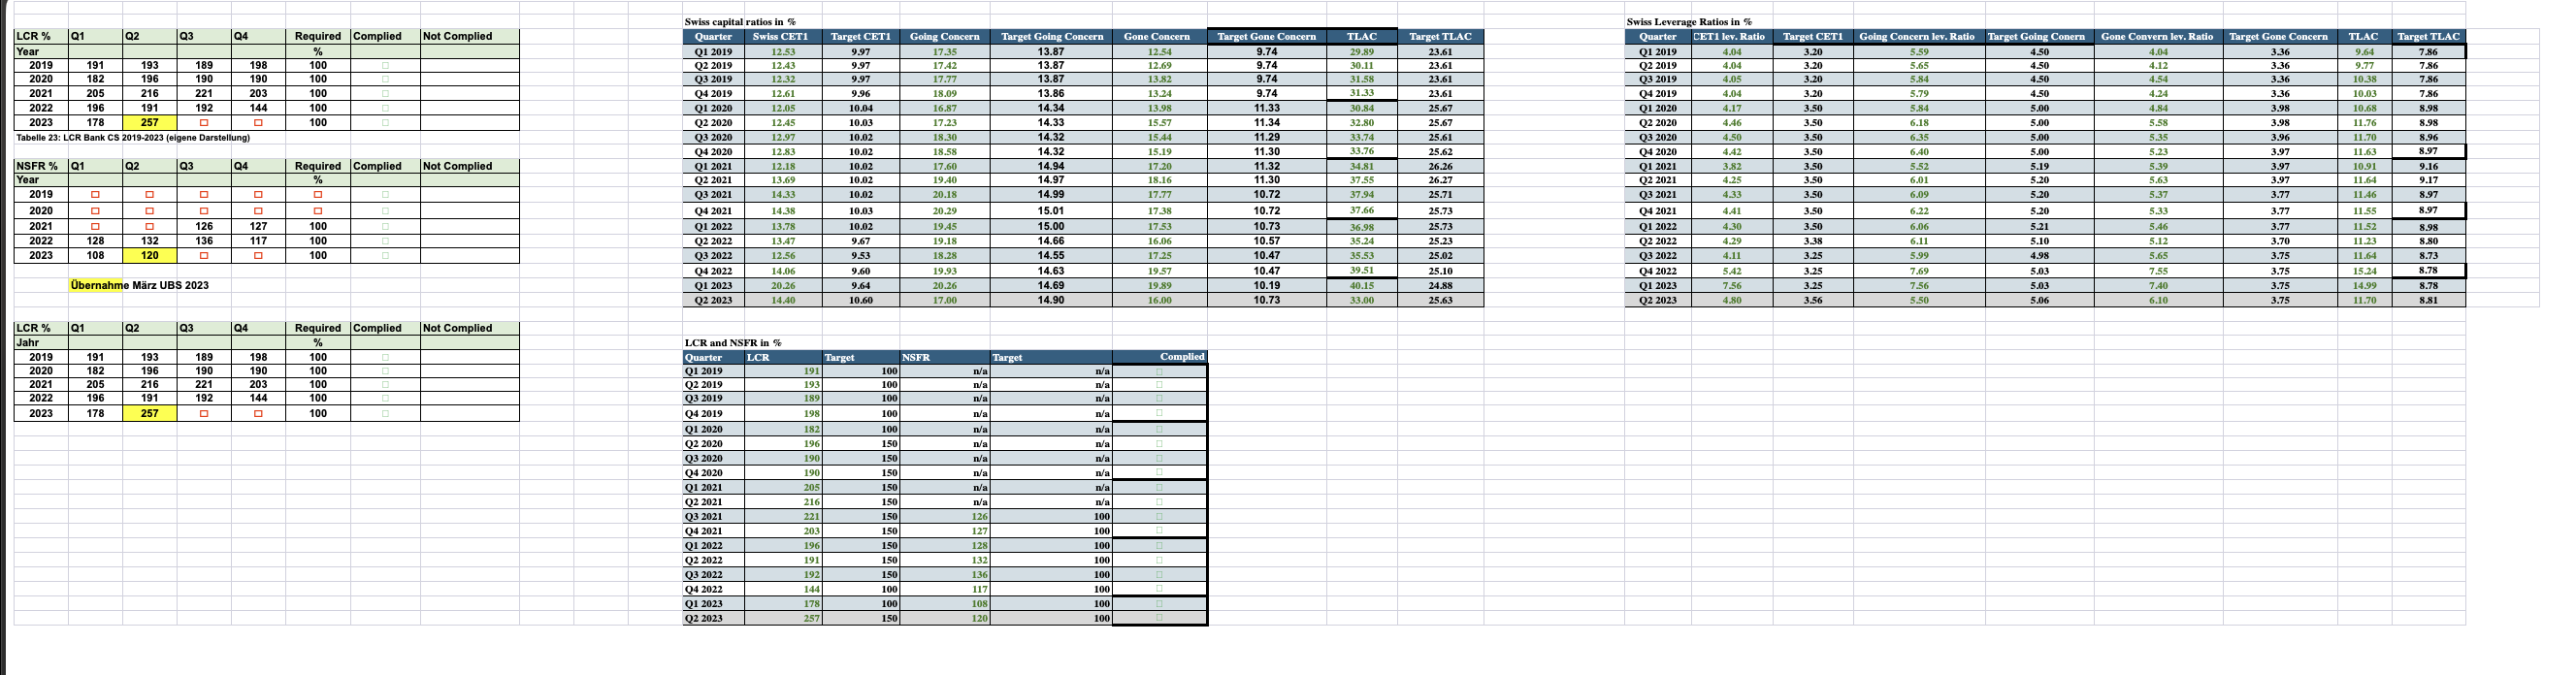
\includegraphics[width=\textwidth]{excel_datengrundlage.png}
  \caption{Datengrundlage aus dem Auftrag (Excel): Kapitalquoten, Leverage Ratios, LCR und NSFR}
  \label{fig:excel}
\end{figure}

\subsection{Anforderungstabelle}
\label{app:anforderungen}
Anforderungen der Aufgabe 2 mit Herkunft im Auftrag (Abschnitt 4 und 5 des Auftragstexts).

{\small
\begin{longtable}{@{}l >{\raggedright\arraybackslash}p{6.2cm} >{\raggedright\arraybackslash}p{6.2cm}@{}}
\toprule
\textbf{ID} & \textbf{Beschreibung} & \textbf{Herkunft im Auftrag} \\
\midrule
\endhead
F1 & Suche über alle drei Inhaltsbereiche (Fälle, Blogs, Organigramm) & „Die Eingabe im bestehenden Suchfeld löst eine Suche über alle drei Inhaltsbereiche aus.“ \\
F2 & Übersichtliche Ergebnisdarstellung mit Kategorie je Treffer & „Ergebnisse werden dem Nutzer übersichtlich dargestellt, inkl. erkennbarer Kategorie je Treffer.“ \\
F3 & Klick auf ein Ergebnis führt zur passenden Seite bzw. zum Eintrag & „Ein Klick auf ein Ergebnis führt zur passenden Seite bzw. zum passenden Eintrag in der Applikation.“ \\
F4 & Berücksichtigung der aktiven Sprache bei den Fallstudien & „Die Suche berücksichtigt die aktuell aktive Sprache: Treffer aus den Fallstudien werden in der jeweils gewählten Sprache gesucht und angezeigt.“ \\
F5 & Sinnvoller Umgang mit Sonderfällen (keine Treffer, kurze Begriffe, leere Eingabe) & „Es existiert ein sinnvoller Umgang mit Sonderfällen: keine Treffer, sehr kurze Suchbegriffe, leere Eingabe.“ \\
F6 & Performante Suche ohne spürbare Verzögerung & „Die Suche funktioniert performant genug für eine flüssige Nutzung.“ \\
F7 & Ergebnisvorschau während der Eingabe & „Ergebnisvorschau während der Eingabe (z.\,B. Dropdown mit Live-Vorschlägen), statt nur nach Bestätigung.“ \\
F8 & Hervorhebung des Suchbegriffs in der Trefferanzeige & „Hervorhebung des gesuchten Begriffs innerhalb der Trefferanzeige.“ \\
F9 & Tippfehler- und Teilstring-Toleranz & „Grundlegende Tippfehler-/Teilstring-Toleranz.“ \\
F10 & Tastaturbedienbarkeit (Pfeiltasten, Enter) & „Tastaturbedienbarkeit (Navigation der Ergebnisliste mit Pfeiltasten, Bestätigung mit Enter).“ \\
N1 & Barrierefreiheit der Ergebnisanzeige (Screenreader) & „Diese Auszeichnung muss bei der Ergebnisanzeige sinngemäss fortgeführt werden.“ \\
N2 & Konsistenz mit bestehenden Code- und Namenskonventionen & „Die Lösung folgt den bestehenden Code- und Namenskonventionen der Applikation.“ \\
N3 & Wartbarkeit: vierter Inhaltsbereich mit vertretbarem Aufwand ergänzbar & „Neue Suchlogik ist so strukturiert, dass ein vierter Inhaltsbereich … ergänzt werden könnte.“ \\
N4 & Sicherheit: serverseitige Behandlung der Nutzereingaben & „Nutzereingaben werden serverseitig korrekt behandelt (keine ungeprüfte Weitergabe an die Datenbank).“ \\
\bottomrule
\end{longtable}
}

\subsection{Verwendete Prompts Aufgabe 1}
\label{app:prompts1}

\subsubsection{Prompt für Prisma}
\textbf{Rohprompt (ohne KI-Hilfe)}
\begin{quote}
\textit{«Ich habe ein Projekt mit Nextjs 16.3, MongoDB, Tailwind 4, Zod 4.4 und Quill 2. Prisma möchte ich mit diesen beiden commands updaten: npm install @prisma/client@6.19 npm install --save-dev prisma@6.19, was können für Fehler passieren? kann ich die Commands einfach aufführen? ist die Kompatibilität okay?»}
\end{quote}

\textbf{Optimierter Prompt}
\begin{lstlisting}
Ich habe ein Next.js-16.3-Projekt mit folgendem Stack: MongoDB als Datenbank (via Prisma), Tailwind CSS 4, Zod 4.4, Quill 2. Aktuell installiert: @prisma/client und prisma in Version 6.17.1.

Ich möchte auf @prisma/client@6.19 und prisma@6.19 (dev) updaten, mit:

npm install @prisma/client@6.19
npm install --save-dev prisma@6.19

Bitte beantworte:
1. Sind diese Befehle für einen MongoDB-Provider unproblematisch, oder gibt es zwischen 6.17.1 und 6.19 relevante Breaking Changes speziell für MongoDB?
2. Muss npx prisma generate danach zwingend erneut laufen?
3. Gibt es bekannte Inkompatibilitäten mit Next.js 16.3 oder mit anderen Paketen in meinem Stack (z.B. @auth/prisma-adapter, @prisma/config)?
4. Welche Tests/Prüfschritte empfiehlst du nach dem Update, gegeben dass im Projekt kein automatisiertes Test-Framework existiert?
5. Worauf sollte ich in der Migrations-/Change-Log-Dokumentation besonders achten, um Risiken für spätere Major-Updates (z.B. Richtung Prisma 7) frühzeitig zu erkennen?

Bitte antworte strukturiert nach diesen 5 Punkten, nicht als Fliesstext.
\end{lstlisting}

\textbf{Vergleich: Was im Rohprompt fehlte}
\begin{center}
\small
\begin{tabularx}{\textwidth}{>{\raggedright\arraybackslash}p{3cm} >{\raggedright\arraybackslash}X >{\raggedright\arraybackslash}X}
\toprule
\textbf{Aspekt} & \textbf{Dein Rohprompt} & \textbf{Was fehlte} \\
\midrule
Ausgangsversion & Nicht genannt (nur Zielversion) & Ohne „von wo“ kann die KI Breaking Changes nicht eingrenzen \\
Verwandte Pakete & @auth/prisma-adapter, @prisma/config nicht erwähnt & Genau diese haben tatsächlich Probleme gemacht (@prisma/config inkompatibel) \\
Antwortformat & Offen („was können für Fehler passieren“) & Ohne Formatvorgabe kommt oft eine unstrukturierte Fliesstext-Antwort, schwer für die Doku verwertbar \\
Testkontext & Nicht erwähnt & Keine automatisierten Tests im Projekt – relevant für sinnvolle Alternativvorschläge (Build/Lint statt Testsuite) \\
Explizite MongoDB-Frage & MongoDB nur als Fakt erwähnt, nicht als gezielte Frage & Die kritischste Erkenntnis (Prisma 7 unterstützt MongoDB nicht) kam erst später – ein gezielter Prompt hätte das evtl. selbst zutage gefördert \\
prisma generate-Frage & Nicht gefragt, obwohl bereits separat ausgeführt & Klärt, ob Reihenfolge/Notwendigkeit stimmt \\
Zukunftsbezug (Prisma 7) & Fehlt komplett & Wichtig, da MongoDB-Inkompatibilität mit Prisma 7 zentral für die Update-Strategie ist \\
\bottomrule
\end{tabularx}
\end{center}

\subsubsection{Prompt für Next.js}
\textbf{Rohprompt (ohne KI-Hilfe)}
\begin{quote}
\textit{«Ich habe ein Projekt mit Nextjs 16.3, MongoDB, Tailwind 4, Zod 4.4 und Quill 2. Wie kann ich das Update machen? Was können für Fehler passieren? Kann ich die Commands einfach aufführen, ist die Kompatibilität okay? Was sind die Breaking Changes? Welche Dinge muss ich sonst noch anpassen ausser der Version in der package.json? Gibt es Tools, die mir dabei helfen können?»}
\end{quote}

\textbf{Optimierter Prompt}
\begin{lstlisting}
Ich habe ein Next.js-Projekt, aktuell auf Version 15.5.9, das ich auf 16.3.2 aktualisieren möchte. Weiterer Stack: React/React-DOM 19.1, MongoDB (via Prisma), Tailwind CSS 4, Zod 4.4, Quill 2, next-auth (Beta), next-intl, next-cloudinary.

Bitte beantworte strukturiert:
1. Vorgehen: Welche Schritte/Befehle sind für ein Next.js-15-auf-16-Update empfohlen (inkl. offizieller Codemod-Tools)?
2. Voraussetzungen: Welche Node.js-Version wird für Next.js 16 mindestens benötigt, und welche React/React-DOM-Version passt dazu?
3. Breaking Changes: Was hat sich zwischen Next.js 15 und 16 grundlegend geändert (z.B. Routing, Middleware, Config-Optionen, Server Components)?
4. Codeanpassungen über die package.json hinaus: Welche Dateien/Konventionen sind typischerweise betroffen (z.B. Umbenennungen wie middleware.ts)?
5. Kompatibilitätsrisiken: Gibt es bekannte Konflikte mit next-auth (Beta), next-intl, next-cloudinary oder Prisma/MongoDB bei diesem Versionssprung?
6. Tools: Welche offiziellen oder Community-Tools (Codemods, Linter-Regeln) unterstützen bei der Migration?
7. Testempfehlung: Wie kann ich das Update verifizieren, wenn im Projekt kein automatisiertes Test-Framework vorhanden ist (nur npm run build / npm run lint)?

Bitte antworte punktuell nach diesen 7 Nummern, nicht als Fliesstext.
\end{lstlisting}

\textbf{Vergleich: Was im Rohprompt fehlte}
\begin{center}
\small
\begin{tabularx}{\textwidth}{>{\raggedright\arraybackslash}p{3cm} >{\raggedright\arraybackslash}X >{\raggedright\arraybackslash}X}
\toprule
\textbf{Aspekt} & \textbf{Dein Rohprompt} & \textbf{Was fehlte} \\
\midrule
Ausgangsversion & Nur Zielversion (16.3) genannt & Ohne „von 15.5.9“ kann die KI den Umfang der Breaking Changes nicht genau eingrenzen \\
Node.js-Version & Nicht erwähnt & Next.js 16 hat eine Mindestanforderung (Node 20.9) – kritisch für CI/Deployment, wäre sonst übersehen worden \\
React-Version & Nicht erwähnt & Next.js 16 verlangt eine bestimmte React-Version-Kompatibilität; ohne diese Angabe bleibt das vage \\
Konkrete Nebenpakete & Nur allgemein „mongodb, tailwind, zod, quill“ & next-auth (Beta!), next-intl, next-cloudinary fehlten – gerade bei next-auth-Beta gibt es reale Kompatibilitätsfragen \\
Antwortformat & Offen & Ohne Strukturvorgabe unübersichtlich für die Doku \\
Testkontext & Nicht erwähnt & Ohne Hinweis auf fehlendes Test-Framework schlägt die KI evtl. unpassende Standardtests vor \\
Copy-Paste-Fehler im ersten Versuch & Prisma-Befehle versehentlich im „Next.js“-Prompt enthalten & Zeigt: beim schnellen Schreiben unter Zeitdruck schleichen sich Kontextvermischungen ein \\
\bottomrule
\end{tabularx}
\end{center}

\subsubsection{Weitere Prompts: Tailwind, Zod, Quill, Cloudinary}
\textbf{Rohprompt (ohne KI-Hilfe)}
\begin{quote}
\textit{«Ich habe ein Projekt mit Nextjs 16.3, MongoDB, Tailwind 4, Zod 4.4 und Quill 2. Wie kann ich das Update von Quill, Tailwind, Zod und Cloudinary machen? Macht es Sinn, alles in einem Prompt zu machen oder einzeln? Was können für Fehler passieren? Was sind die Breaking Changes?»}
\end{quote}

\textbf{Optimierter Prompt}
\begin{lstlisting}
Ich habe ein Next.js-16.3-Projekt mit MongoDB (via Prisma). Folgende Pakete möchte ich aktualisieren, jeweils aktuell installierte Version:
- Tailwind CSS: 4.1.14 (+ @tailwindcss/postcss, @tailwindcss/typography, @tailwindcss/line-clamp, tailwindcss-animate)
- Zod: 4.1.12
- Quill: 2.0.3
- Cloudinary: cloudinary 2.8.0 + next-cloudinary 6.17.5

Nutzungskontext im Projekt: Cloudinary für Bild-Upload, Quill als Rich-Text-Editor, Zod für Schema-Validierung, Tailwind als CSS-Framework mit mehreren Plugins.

Bitte beantworte strukturiert pro Paket:
1. Aktuelle stabile Zielversion
2. Ob es sich um ein Minor/Patch- oder Major-Update handelt
3. Relevante Breaking Changes seit der genannten Ausgangsversion
4. Bekannte Kompatibilitätsrisiken mit Next.js 16.3 oder untereinander (z.B. Tailwind-Plugins mit Tailwind-Core-Version)

Danach:
5. Empfiehlst du, diese vier Pakete in einem Zug oder einzeln nacheinander zu aktualisieren – und warum?
6. In welcher Reihenfolge, falls einzeln?
7. Wie kann ich das Update pro Paket verifizieren, wenn im Projekt kein automatisiertes Test-Framework existiert (nur npm run build / npm run lint)?

Bitte antworte nummeriert nach diesen Punkten, nicht als Fliesstext.
\end{lstlisting}

\textbf{Vergleich: Was im Rohprompt fehlte}
\begin{center}
\small
\begin{tabularx}{\textwidth}{>{\raggedright\arraybackslash}p{3cm} >{\raggedright\arraybackslash}X >{\raggedright\arraybackslash}X}
\toprule
\textbf{Aspekt} & \textbf{Dein Rohprompt} & \textbf{Was fehlte} \\
\midrule
Ausgangsversionen der Pakete & Nur Next.js-Version genannt, nicht die der vier Zielpakete & Ohne genaue Ist-Versionen kann die KI nicht sagen, ob es sich um einen Major- oder Minor-Sprung handelt \\
Zusatzpakete/Plugins & Nicht erwähnt & Tailwind hat mehrere Zusatzpakete, Cloudinary besteht aus zwei Paketen – sonst driften Versionen auseinander \\
Nutzungskontext & Fehlt & Ohne zu wissen, wofür die Pakete verwendet werden, kann die KI nur generische statt projektspezifische Risiken nennen \\
Reihenfolge-Frage konkretisiert & Nur „alles in einem oder einzeln“ gefragt & Die logische Folgefrage „in welcher Reihenfolge“ fehlte \\
Antwortformat & Offen & Bei vier Paketen gleichzeitig besonders wichtig, sonst vermischen sich die Aussagen \\
Testkontext & Nicht erwähnt & Gleiches wiederkehrendes Muster wie bei den vorherigen zwei Prompts \\
\bottomrule
\end{tabularx}
\end{center}

\subsection{Anleitung Next.js-Update auf 16.3.2}
Die Aktualisierung erfolgte in dieser Reihenfolge (Vorgaben aus dem Auftrag, Stand der Versionen siehe Versionsübersicht in Kapitel 3):
\begin{enumerate}[nosep]
  \item \textbf{Voraussetzung:} Node.js ab Version 20.9 in Entwicklung und Deployment. Next.js 16 verlangt mindestens diese Version.
  \item \textbf{Prisma zuerst:} \texttt{npm install @prisma/client@6.19} und \texttt{npm install --save-dev prisma@6.19}. CLI und Client müssen dieselbe Version haben. Danach \texttt{npx prisma generate}. Die ungenutzte Abhängigkeit \texttt{@prisma/config} wird mit \texttt{npm uninstall @prisma/config} entfernt, weil sie nicht zu Prisma 6 passt. Prisma 7 unterstützt MongoDB nicht.
  \item \textbf{Offizieller Codemod:} \texttt{npx @next/codemod@canary upgrade latest}.
  \item \textbf{Versionen anheben:} Next.js auf 16.3.2, React und React-DOM auf 19.2.8 (gemeinsam mit Next.js) und \texttt{eslint-config-next} auf 16.3.2.
  \item \textbf{Middleware migrieren:} \texttt{middleware.ts} wird zu \texttt{proxy.ts}, mit \texttt{npx @next/codemod@canary middleware-to-proxy}. Danach waren zwei Stellen von Hand zu korrigieren: \texttt{page} muss neu als zweiter Parameter übergeben werden, und die \texttt{.env}-Datei musste angepasst werden.
  \item \textbf{Weitere Pakete:} \texttt{next-cloudinary} auf 6.18.8, danach Tailwind CSS, Zod, Quill und Cloudinary.
  \item \textbf{Prüfung:} \texttt{npm run dev}, \texttt{npm run build} und \texttt{npm run lint} ausführen und die Seiten von Hand im Browser testen.
\end{enumerate}

\subsection{Prompts und Plan Aufgabe 3}
Den Umsetzungsplan (\texttt{todo/plan.md}) hat Claude Code aus dem Auftrag und den drei Mockups erstellt. Die Fragen und Antworten stehen in \texttt{todo/questions-answers.md}. Meine Eingaben dazu (im Wortlaut, auf Englisch):
\begin{lstlisting}
1. "create a plan as markdown file for the task.md file with the steps to modify the code, 3 images are in the folder todo, image003, image006, image007 use them as input, if you are unsure ask questions in stead f guessing"

2. Antworten auf die Rueckfragen:
   - Daten: "Show the excerpt only"
   - Sprachen: "All 5 via messages"
   - Slugs: "how is the site currently handling it, with the blogs, they probalby have diffrent slug per langauge"
   - SEO/Suche: "Sitemap + search"
   - Tabelle 6: "Use the 3 visible values"

3. "doc ument the answers and questions in a doc file"
4. "make a markdown in the todo folder"
5. Manuelle Ergaenzung im Plan, offener Punkt 3: "-> beispiel content erstellen"
6. "how can the plan.md be worked on in parrallel?"
7. "write that in the plan so the agents can work in parrallel"
8. "comppress the contnet of this chat into a very short file, with what happend and put that in the folder aswell as an md file"
9. "also add my inputs to the file"
\end{lstlisting}

\subsection{Zugriff auf Code}
Repository: \url{https://github.com/mrexito/CS-UBS_update} \\
Branches: \texttt{main}, \texttt{upgrade/next16-prisma7}, \texttt{search-feature}, \texttt{rc/*} \\
Start der App: \texttt{npm install}, danach \texttt{npm run dev} (Entwicklungsserver, Standard \url{http://localhost:3000}). Voraussetzungen sind Node.js ab Version 20.9 und eine \texttt{.env}-Datei mit den Schlüsseln, die der Auftraggeber bereitgestellt hat. Produktions-Build mit \texttt{npm run build}, API-Tests der Suche mit \texttt{npm run test:search} (benötigt laufenden Entwicklungsserver).

\end{document}
